\section{Results \& Discussion}
%MSE, RMSE, MAE , PCA, R2, compair.
%Ordered by target:

The accuracy of the ML method in this work is evaluated using R-squared ($R^2$), "Mean" of the training target values, standard deviation (stdev) of the error, mean absolute error (MAE), root-mean-square-error (RMSE) and weighted absolute percentages error (WAPE), as described in \ref{sec:evaluation_method}. Lower RMSE, MAE, and WAPE, with a high $R^2$-score indicate a better ML prediction. The overall performance of the model was evaluated using the k-fold cross-validation technique for 10 folds \ref{sec:cross_validation}, and is referred to as $R^2$ - cross-validation mean or $R^2$-CVM.
Before each run a PCA is performed and the PCs that collectively accounted for $99\%$ of the variation are selected for the RF run, the last $1\%$ of the variation, i.e. the other predictors, are removed.

For each intercalation battery type, both Mg-ion and Li-ion, four different sets of descriptors are reported, namely:

\begin{itemize}
\item Material specific properties
\item Volumetric number density 
\item Void fraction
\item APRDF
\end{itemize}


The targets the suggested features are tested on are: \textbf{Average Voltage} (\ac{AV}), \textbf{Gravimetric Capacity} (\ac{GC}), \textbf{Volumetric Capacity} (\ac{VC}), \textbf{Specific Energy} (\ac{SE}), and \textbf{Energy Density} (\ac{ED}). First, the set of descriptors were individually tested. Afterwards, they were combined to make the best possible classifier.

\subsection{Target distribution}

From the target distributions in figure \ref{fig:Mg_targets_a-e} and \ref{fig:Li_targets_a-e}, we can see that the Li-ion db has more data, but also stronger outliers. An example of outlier from the Li-ion db, there are $11$ batteries with an AV between $6-\SI{9}{V}$ in the db, or the single material with a specific energy between $2500 \& 3000 \text{ } \si{Wh/kg}$. Except for the outliers are the distribution of AV even for both databases, with most values in the range of $1-5$. This trend, of similar distribution seems valid for SE and ED, which seems curious due to Li metal having a higher SE. While GC and VC seems to be lower for Li-ion batteries in general. 

As a note on the target data, GC and VC, as well as SE and ED are different representations of the same characteristic in the battery. The reason for using both as targets is to evaluate how our ML model differs between these dataset.
%Mg
 \begin{figure}[h]
     \centering
     \begin{subfigure}{0.3\textwidth}
         \centering
         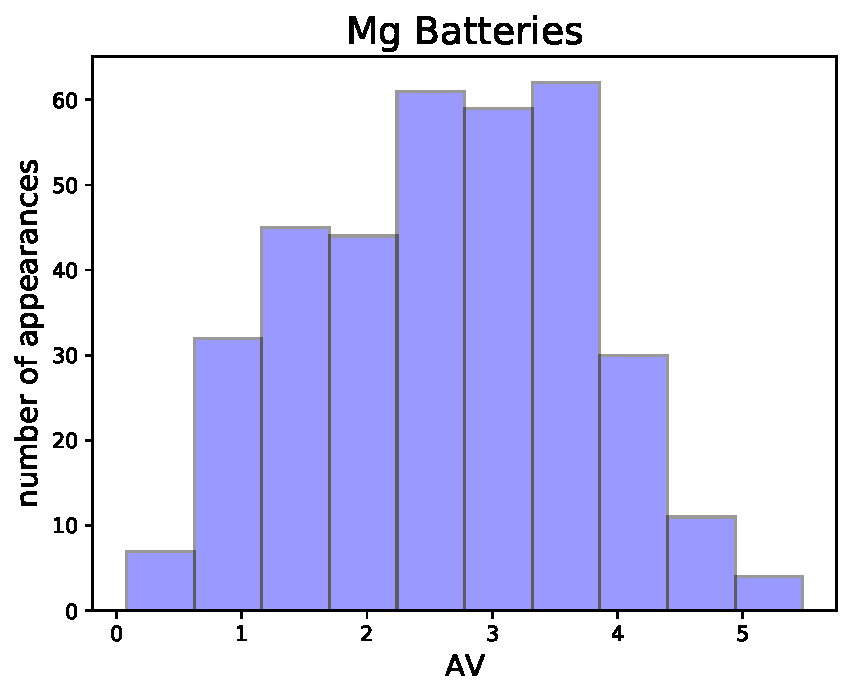
\includegraphics[width=\linewidth]{result/figures/columnsplotMg_AV.pdf}
         \caption{}
     \end{subfigure}
     ~ 
     \begin{subfigure}{0.3\textwidth}
         \centering
         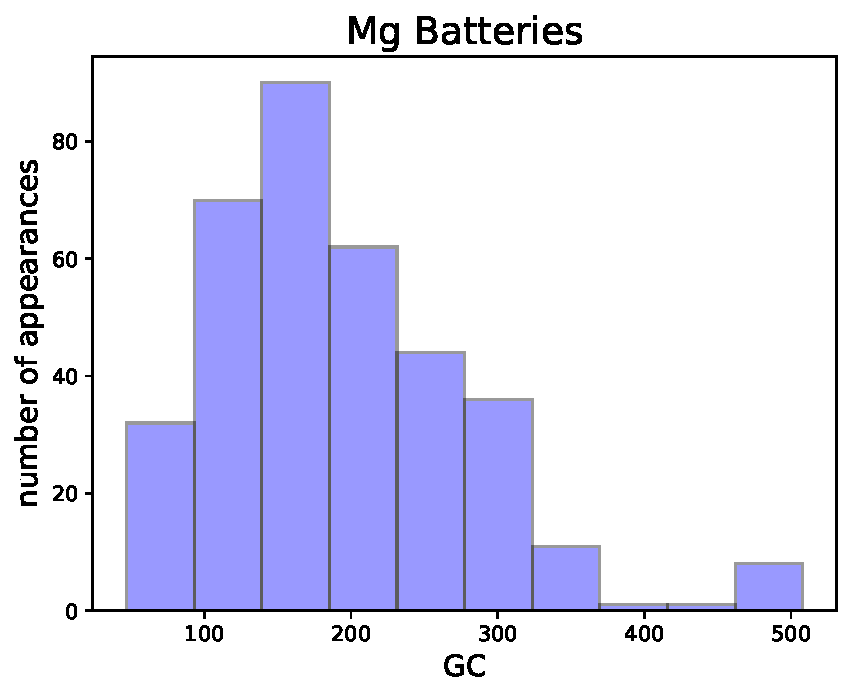
\includegraphics[width=\linewidth]{result/figures/columnsplotMg_GC.pdf}
         \caption{}
     \end{subfigure}
          ~ 
     \begin{subfigure}{0.3\textwidth}
         \centering
         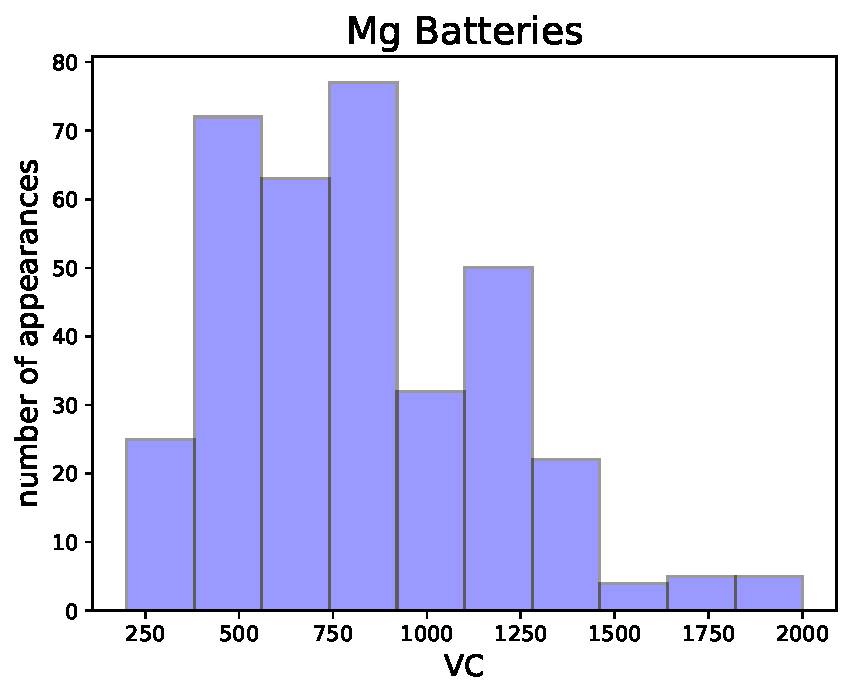
\includegraphics[width=\linewidth]{result/figures/columnsplotMg_VC.pdf}
         \caption{}
     \end{subfigure}
          ~ 
     \begin{subfigure}{0.3\textwidth}
         \centering
         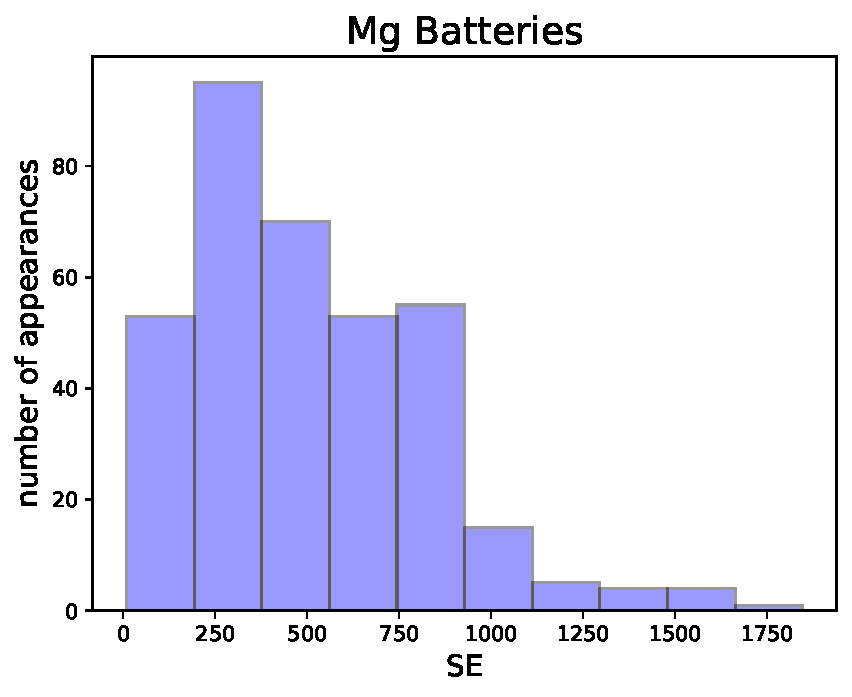
\includegraphics[width=\linewidth]{result/figures/columnsplotMg_SE.pdf}
         \caption{}
     \end{subfigure}
          ~ 
     \begin{subfigure}{0.3\textwidth}
         \centering
         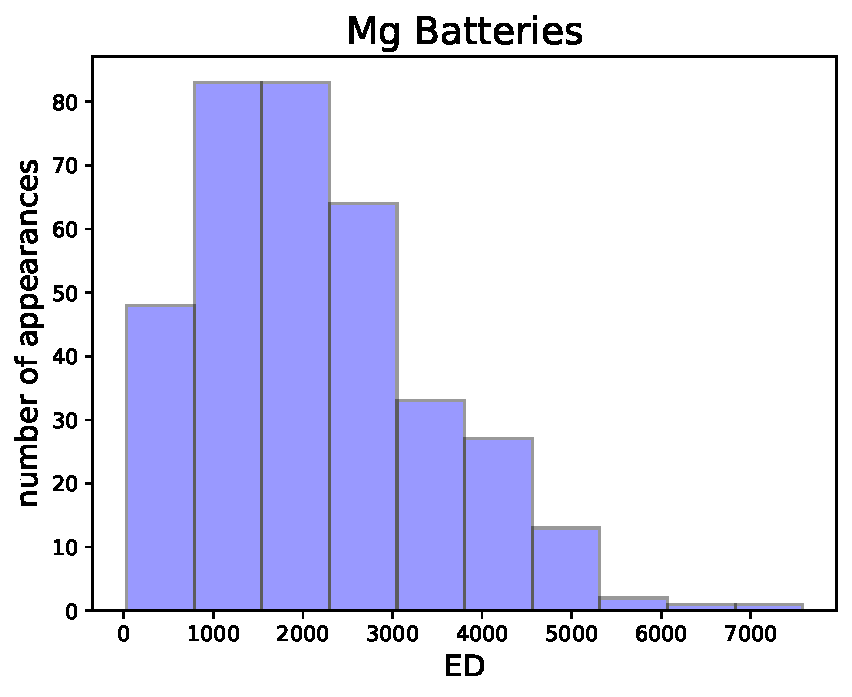
\includegraphics[width=\linewidth]{result/figures/columnsplotMg_ED.pdf}
         \caption{}
     \end{subfigure}
     \caption{a)-e) are the distribution of the targets Average Voltage, Gravimetric Capacity, Volumetric Capacity, Specific Energy and Energy Density, for the Mg-ion database. The x-axis are the target values and the y-axis are the number of appearances for that range of target values.}
     \label{fig:Mg_targets_a-e}
 \end{figure}
%Li
 \begin{figure}[h]
     \centering
     \begin{subfigure}{0.3\textwidth}
         \centering
         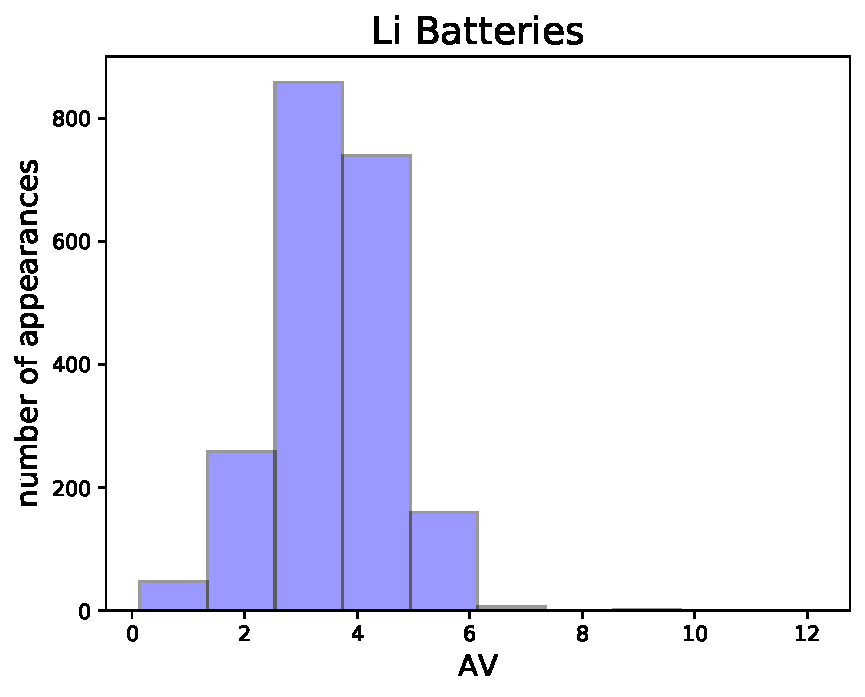
\includegraphics[width=\linewidth]{result/figures/columnsplotLi_AV.pdf}
         \caption{}
     \end{subfigure}
     ~ 
     \begin{subfigure}{0.3\textwidth}
         \centering
         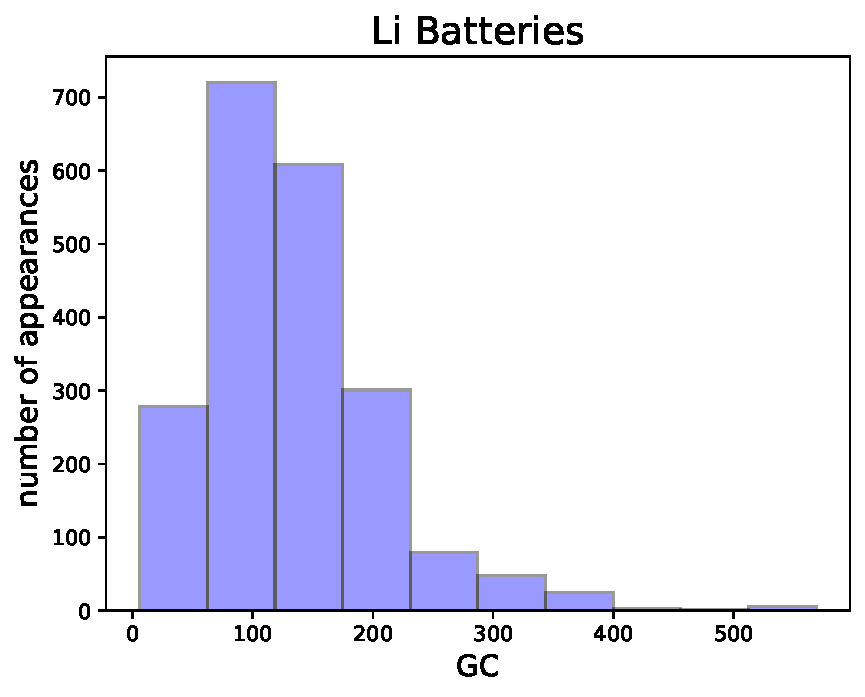
\includegraphics[width=\linewidth]{result/figures/columnsplotLi_GC.pdf}
         \caption{}
     \end{subfigure}
          ~ 
     \begin{subfigure}{0.3\textwidth}
         \centering
         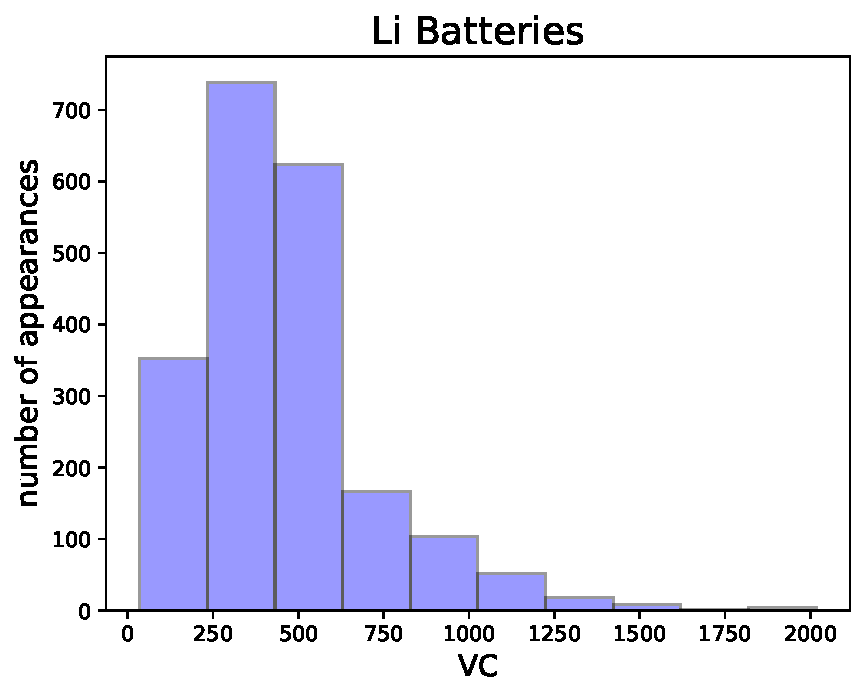
\includegraphics[width=\linewidth]{result/figures/columnsplotLi_VC.pdf}
         \caption{}
     \end{subfigure}
          ~ 
     \begin{subfigure}{0.3\textwidth}
         \centering
         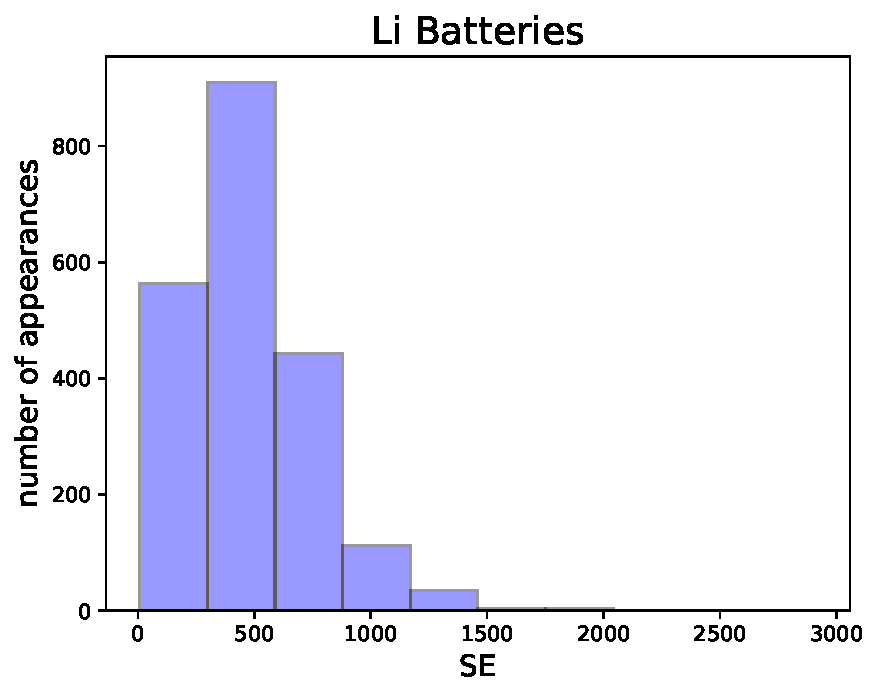
\includegraphics[width=\linewidth]{result/figures/columnsplotLi_SE.pdf}
         \caption{}
     \end{subfigure}
          ~ 
     \begin{subfigure}{0.3\textwidth}
         \centering
         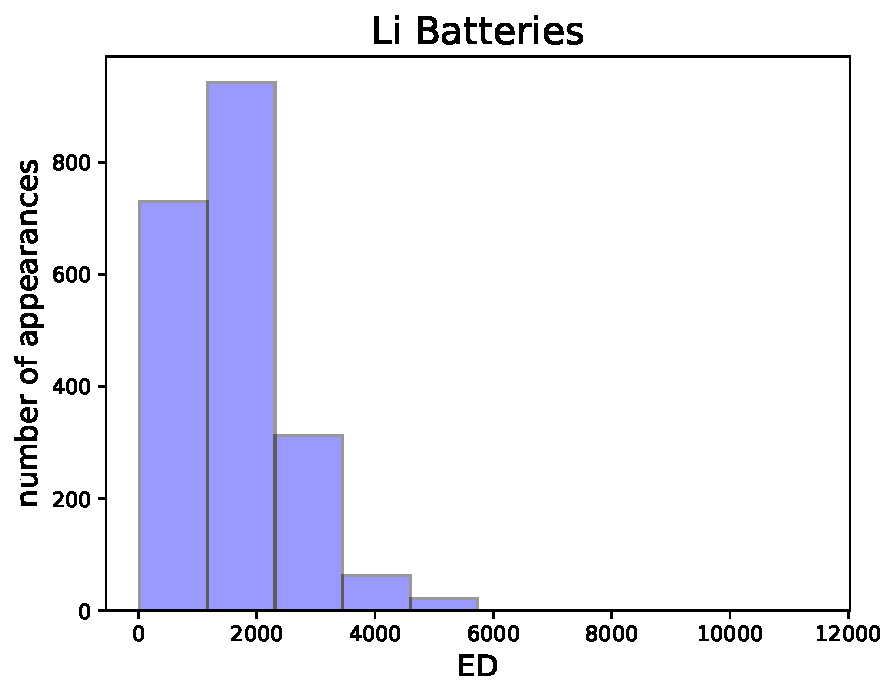
\includegraphics[width=\linewidth]{result/figures/columnsplotLi_ED.pdf}
         \caption{}
     \end{subfigure}
     \caption{a)-e) are the distribution of the targets: Average Voltage, Gravimetric Capacity, Volumetric Capacity, Specific Energy and Energy Density, for the Li-ion database. The x-axis are the target values and the y-axis are the number of appearances for that range of target values.}
     \label{fig:Li_targets_a-e}
 \end{figure}



\FloatBarrier
\subsection{Size of database, and number of estimators}
	There are two hyper-parameters that need to be adjusted when using random forest. These are the number of estimators and the maximum number of features. The number of estimators are the sum of decision trees used in the forest. The optimal amount of trees used for the model is a compromise between predicational quality and computational cost: The more trees, the better the prediction, but the model becomes more computationally expensive. However, the improvement rate will slow down after a critical number of trees. To find the optimal number of trees for our predictions, we made several model using $5,10,25,50,100,250,500,1000$ decision trees, creating $10$ unique forests for each amount of trees and plottet them with the standard deviation of the $10$ runs. The results, for both databases can be seen in figure \ref{fig:trees_size}. We decided to use $250$ estimators, this gave a good compromise between cost and accuracy. It could be argued that applying $100$ estimators is sufficient for an accurate prediction, but the computational impact is not noticeable for a database of this size, so opting in to a possible improvement is favored. 
	 For the latter, the number of selected features can influence the generalization error by: Applying few features, reducing the number of trees to lower correlation among the trees, leading to a stronger forest. Or selecting many features, increasing the strength of each individual tree. In Breiman's paper on RF \cite{breiman2001random} it is recommended to apply $N/3$ features per split, with $N$ features. While in the paper "Extremely randomized trees" by Geurts \textit{et al.} it was empirically justified to used all features \cite{geurts2006extremely}. Our random forest regressor always considers all features instead of a random subset of features, due to Geurts paper, and the paper by Shandiz \textit{et al.} \cite{shandiz2016application} showing to higher accuracy by applying all features.


\begin{figure}[h]
    \centering
    \begin{subfigure}{0.45\textwidth}
        \centering
        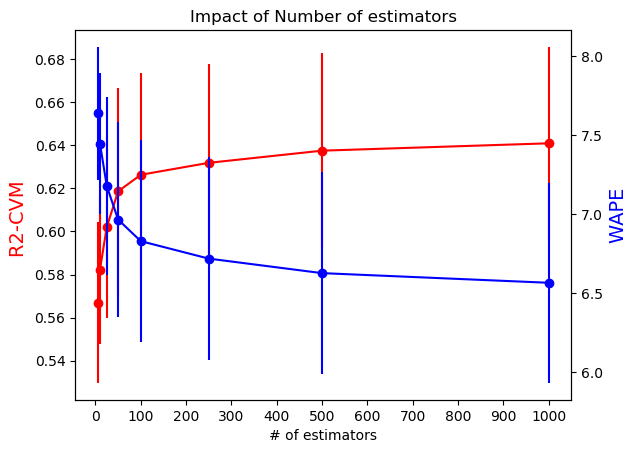
\includegraphics[width=\linewidth]{result/figures/Mg_n_estimators-2.png}
        \caption{Mg}
        \label{fig:Mg_n_estimators}
    \end{subfigure}%
    ~ 
        \begin{subfigure}{0.45\textwidth}
        \centering
        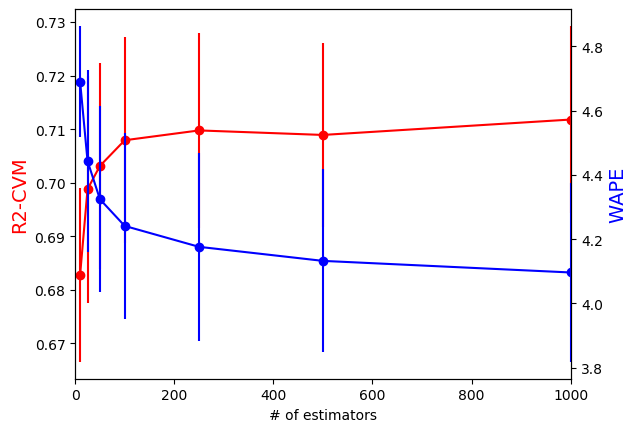
\includegraphics[width=\linewidth]{result/figures/Li_number_of_estimators-4.png}
        \caption{Li}
        \label{fig:Li_size_db}
    \end{subfigure}
	\caption{The number of estimators used plottet vs. $R^2-CVM$ and WAPE. The predictions are done with the same combination of features as in table \ref{tab:Li-vnd-msp-vf-stability}, with Average Voltage as the target.}
	\label{fig:trees_size}
\end{figure}


The two data sets are of different size. The Mg-ion database (\ac{db}) has $355$ different batteries, while the Li-ion db has $2073$ different Li batteries, more than five times the size of the Mg-ion db. Both of these databases are relative small from a ML perspective, but are large enough to show correlations. 

Impact of the size of our dataset was tested using $10\%,20\%,...,100\%$ of our database. Our data were split into two parts, the training data $X_{\text{train}}, 80\%$, and the test data, $X_{\text{test}},20\%$. Each of these calculations were done $10$ times for all unique percentage. The mean of $R^2$-CVM and WAPE was plottet with their respective standard deviations against the percentage of the database used, as seen in figure \ref{fig:trees_size}. The Li-ion db was also tested for $5\%$ of the db, utilizing $103$ Li-ion batteries, almost the same as $30\%$ of the Mg-ion db. This was not feasible for the Mg-ion db, since $5\%$ makes up $17$ batteries, and it makes the ML model very unreliable, as can be seen from the $10\%$, and $20\%$ in figure \ref{fig:trees_size}.

\begin{figure}[h]
    \centering
        \begin{subfigure}{0.45\textwidth}
        \centering
        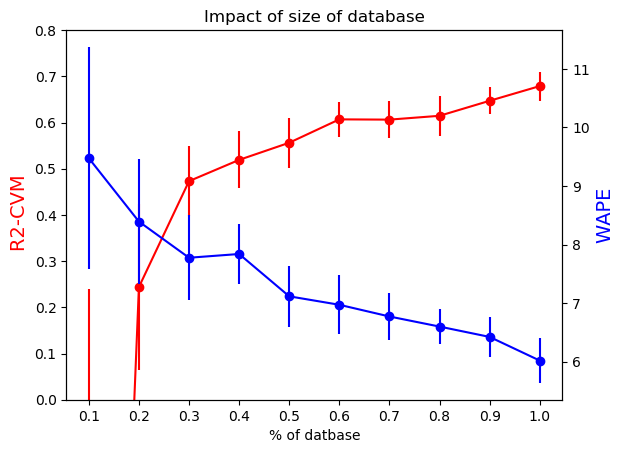
\includegraphics[width=\linewidth]{result/figures/Mg_size_db-2.png}
        \caption{Mg}
        \label{fig:Mg_size_db}
    \end{subfigure}
    ~ 
        \begin{subfigure}{0.45\textwidth}
        \centering
        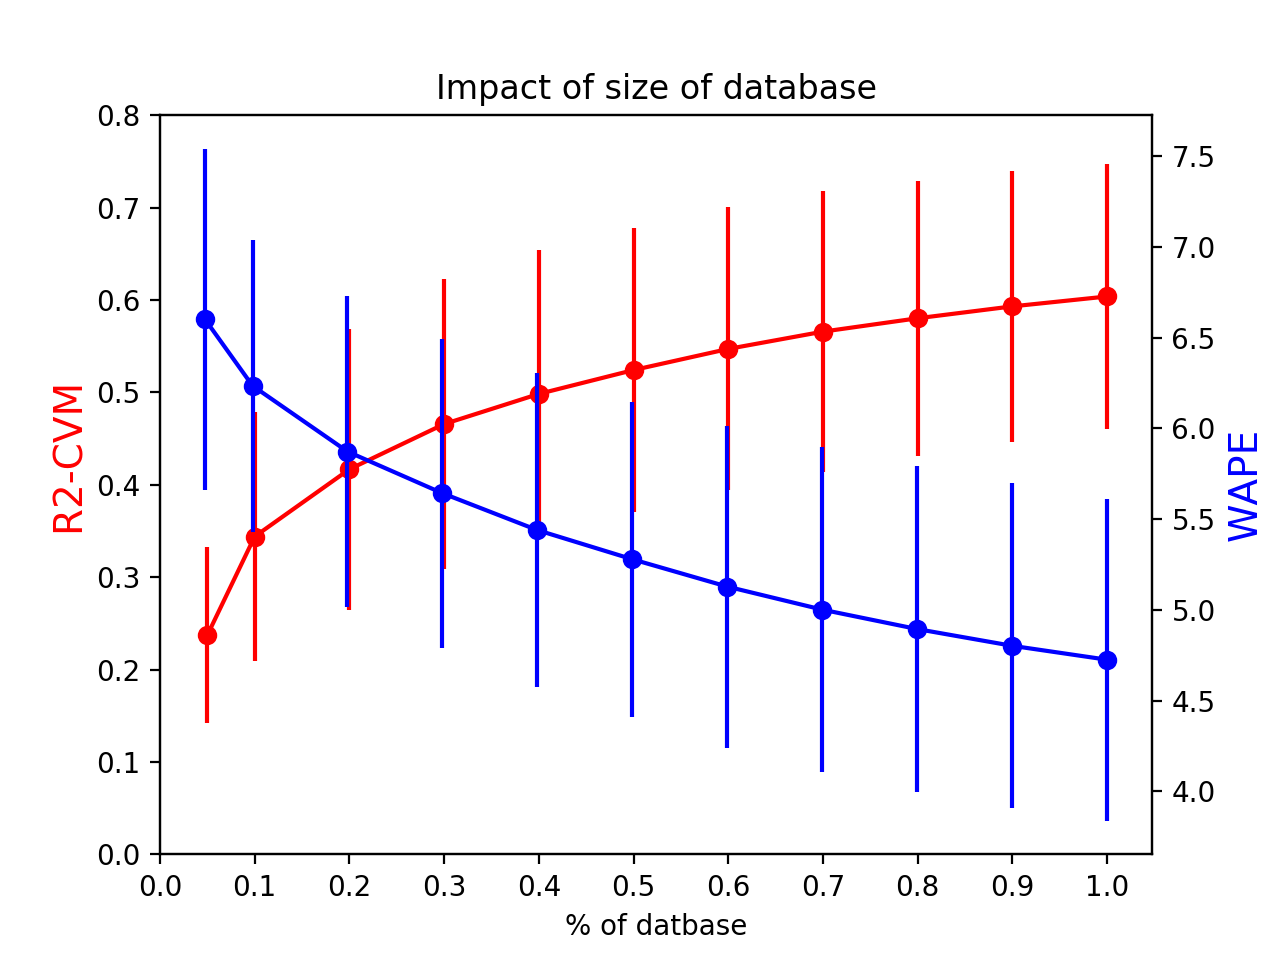
\includegraphics[width=\linewidth]{result/figures/Li_size_db-2.png}
        \caption{Li}
        \label{fig:Li_size_db}
    \end{subfigure}
	\caption{Indicates the impact of the size of the database. Percentage of the database is plottet vs. $R^2-CVM$ and WAPE. The predictions are done with the same combination of features as in table \ref{tab:Li-vnd-msp-vf-stability}, with Average Voltage as the target.}
	\label{fig:trees_size}
\end{figure}


	An example of a PCA run on our data, as explained in section \ref{sec:PCA}, are shown in figure\ref{fig:PCA_dim}. We found that we could reduce the dimensionality of our two datasets (figure \ref{fig:PCA_dim}), when applying all features, with $38.9\%$ and $57.0\%$ for the Mg-ion and Li-ion databases respectively, that is a reduction of $29$ out of $72$, and $70$ out of $124$ applied features. 
		
\begin{figure}[H]
    \centering
    \begin{subfigure}{0.48\textwidth}
        \centering
        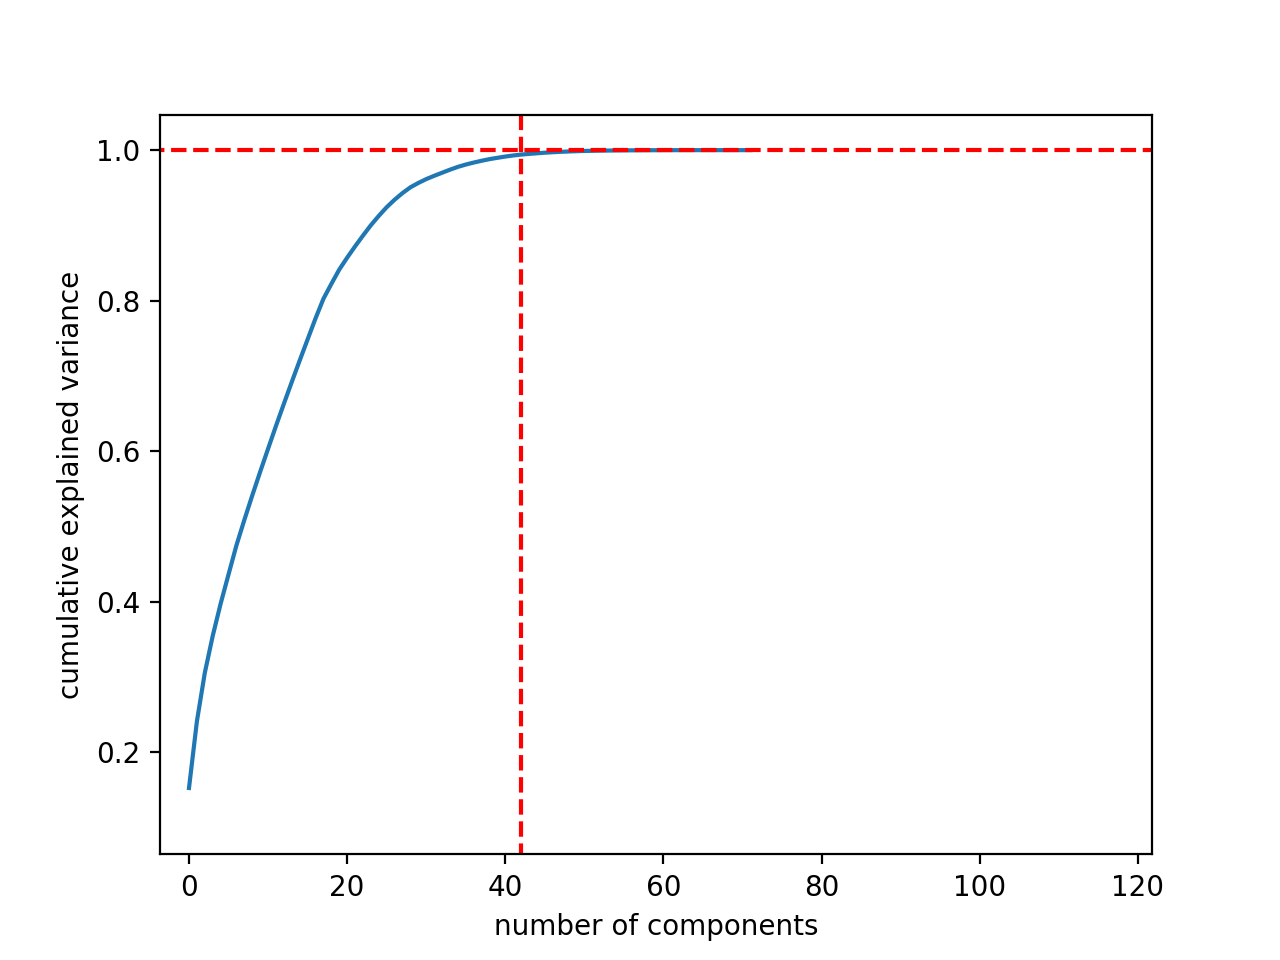
\includegraphics[width=\linewidth]{theory/figures/Mg_PCA.png}
        \caption{Mg}
        \label{fig:PCA_b}
    \end{subfigure}
        ~ 
    \begin{subfigure}{0.48\textwidth}
        \centering
        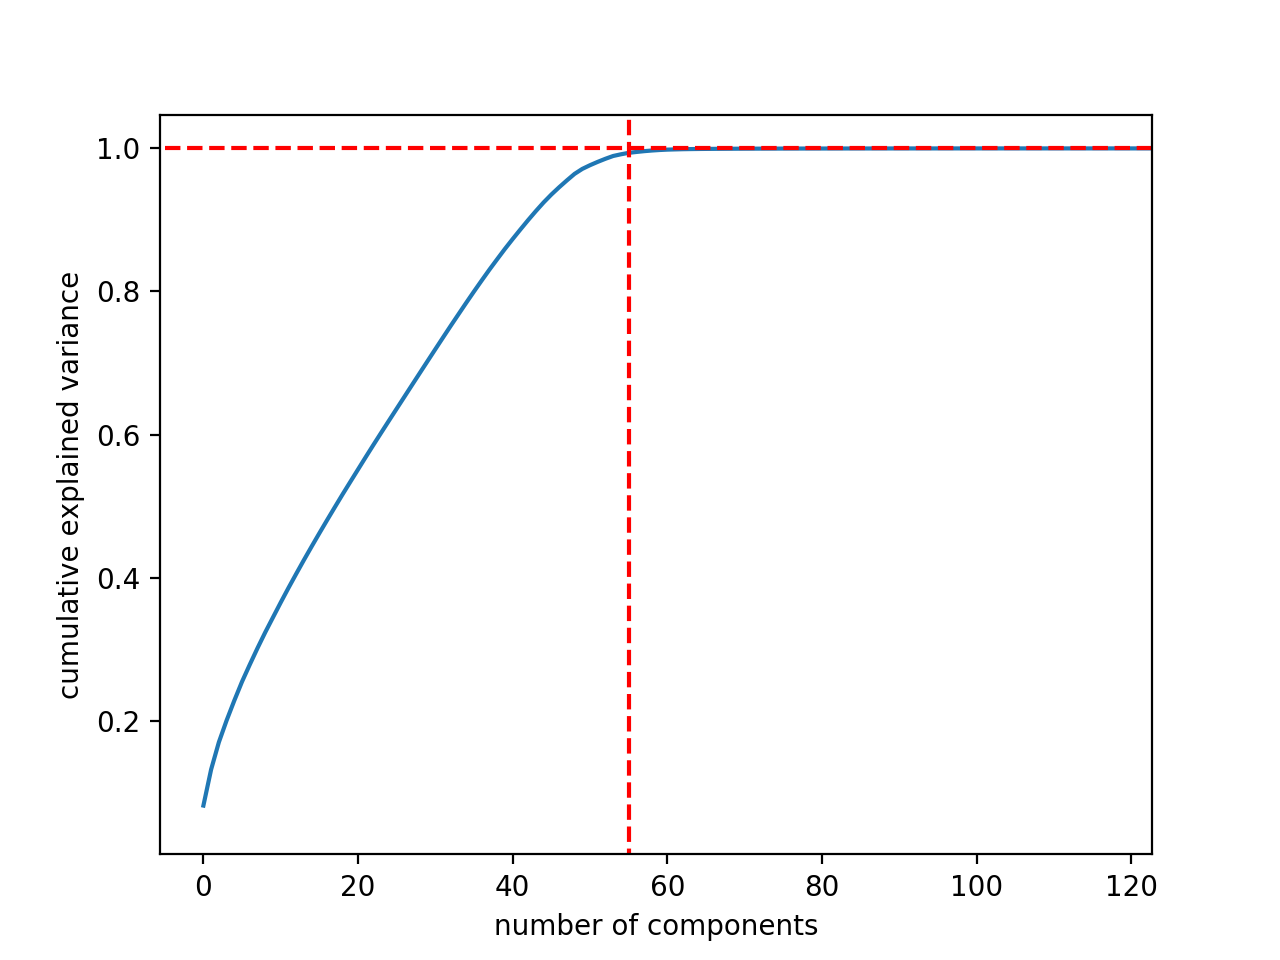
\includegraphics[width=\linewidth]{theory/figures/PCA_reduction_of_dimensionality.png}
        \caption{Li}
        \label{fig:PCA_a}
    \end{subfigure}%
	\caption{Principal component analysis for the feature vectors leads to a reduction of: a) $40.2\%$ of the dimensionality, removing $29$ features from the $72$ predictions applied to the Mg-ion database. And b) $56.0\%$ of the dimensionality, removing $70$ of the $124$ features form the prediction applied to the Li-ion database.}
	\label{fig:PCA_dim}
\end{figure}
 


  
\subsection{Material specific properties}
The \textit{material specific properties} (\ac{msp}), are the properties related to every individual material, both charged and discharged. They are; \textbf{energy, energy per atom, volume of the unit cell, band gap, density, magnetization, number of sites}, and \textbf{elasticity}, for both the charged and discharged material, as explained in section \ref{sec:theory_bat}. Evaluation of \textbf{stability} (stab) from the MP db will be included in this section, but will be treated as its own group of features. The Materials Project database included \textbf{formation energy per atom} for most structures, but due to "None" values and no significant change in our predictions. It is likely that any given decision tree with variables containing zeros will be ignored by the algorithm unless they facilitate some other correlation. Therefor it was decided to leave these features out of our predictions. We will first have a look at the distribution of our prediction.

%----------------------------------------------------------------------------------------------------
Figure \ref{fig:Mg_msp_distribution} shows the distribution for the msp, for charged materials in green and discharged materials in red. The two battery materials tends to have the same type of distribution and therefore it is interesting to see that one of the two features are commonly not dismissed, it is rather the feature as a whole that is deemed dispensable by the ML model.  

\begin{figure}[h]
     \centering
          \begin{subfigure}{0.2\textwidth}
         \centering
         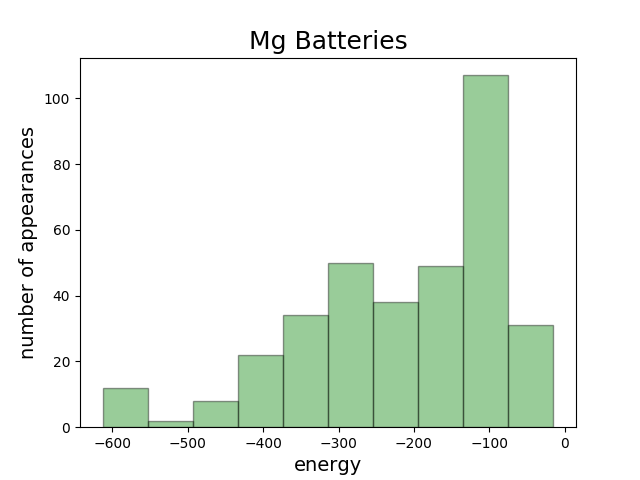
\includegraphics[width=\linewidth]{result/figures/distribution/Mg_distrof_energy.png}
         
     \end{subfigure}
     ~ 
     \begin{subfigure}{0.2\textwidth}
         \centering
         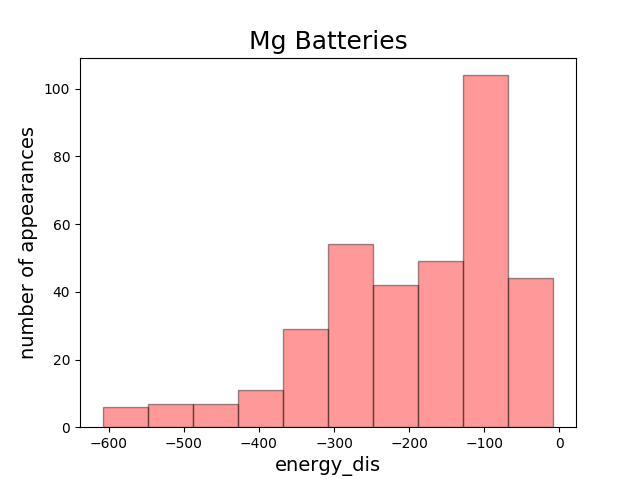
\includegraphics[width=\linewidth]{result/figures/distribution/Mg_distrof_energy_dis.png}
         
     \end{subfigure}
          ~ 
     \begin{subfigure}{0.2\textwidth}
         \centering
         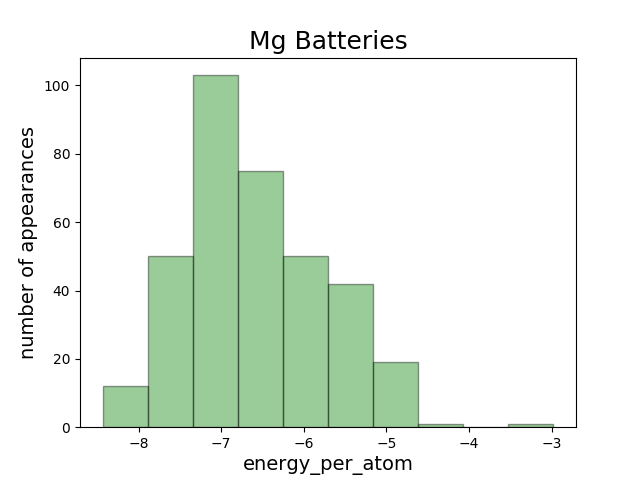
\includegraphics[width=\linewidth]{result/figures/distribution/Mg_distrof_energy_per_atom.png}
         
     \end{subfigure}
     ~ 
     \begin{subfigure}{0.2\textwidth}
         \centering
         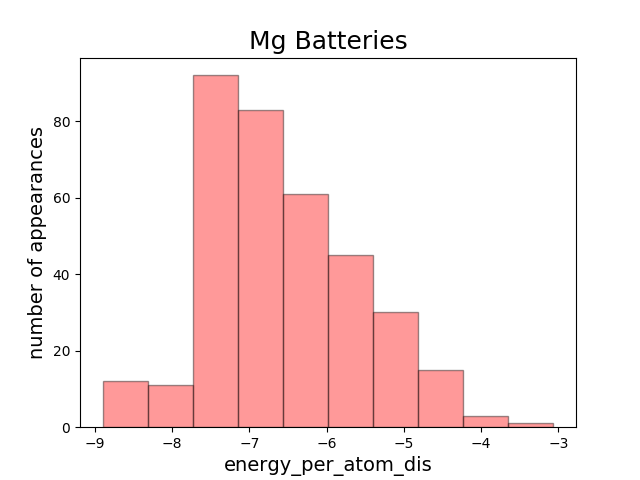
\includegraphics[width=\linewidth]{result/figures/distribution/Mg_distrof_energy_per_atom_dis.png}
         
     \end{subfigure}
          ~ 
     \begin{subfigure}{0.2\textwidth}
         \centering
         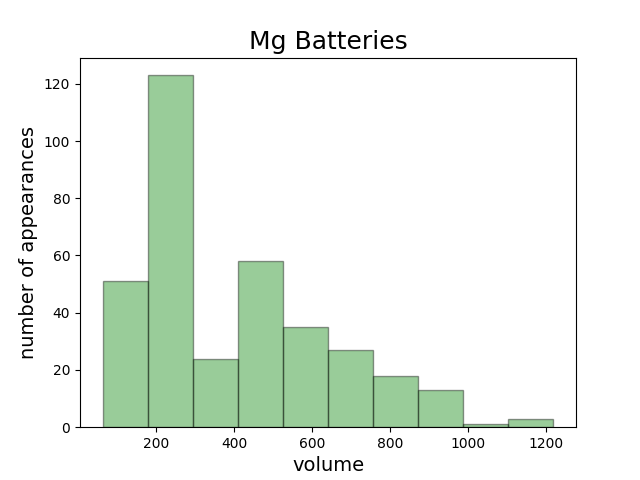
\includegraphics[width=\linewidth]{result/figures/distribution/Mg_distrof_volume.png}
         
     \end{subfigure}
          ~ 
     \begin{subfigure}{0.2\textwidth}
         \centering
         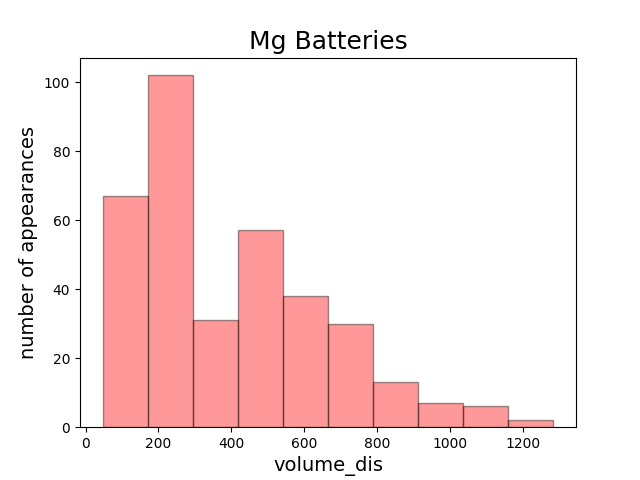
\includegraphics[width=\linewidth]{result/figures/distribution/Mg_distrof_volume_dis.png}
         
     \end{subfigure}
          ~ 
         \begin{subfigure}{0.2\textwidth}
         \centering
         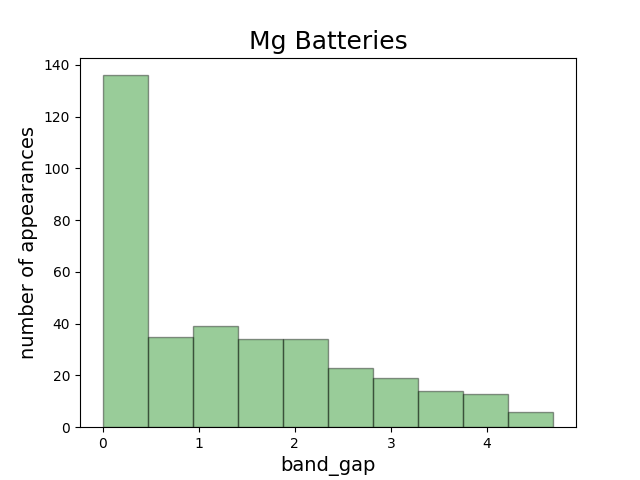
\includegraphics[width=\linewidth]{result/figures/distribution/Mg_distrof_band_gap.png}
         
     \end{subfigure}
          ~ 
     \begin{subfigure}{0.2\textwidth}
         \centering
         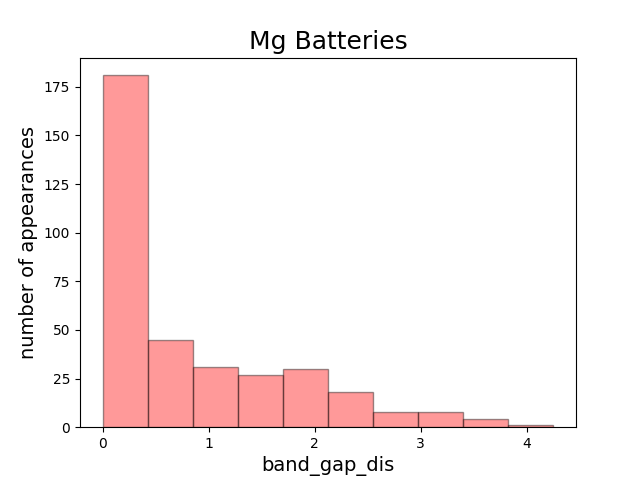
\includegraphics[width=\linewidth]{result/figures/distribution/Mg_distrof_band_gap_dis.png}
         
     \end{subfigure}
          ~ 
               \begin{subfigure}{0.2\textwidth}
         \centering
         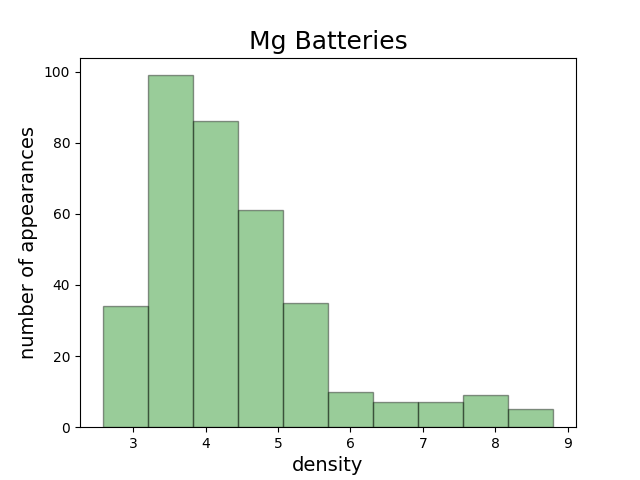
\includegraphics[width=\linewidth]{result/figures/distribution/Mg_distrof_density.png}
         
     \end{subfigure}
          ~ 
     \begin{subfigure}{0.2\textwidth}
         \centering
         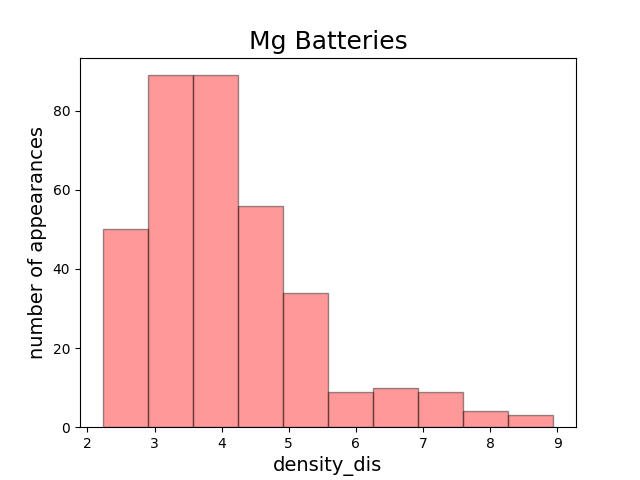
\includegraphics[width=\linewidth]{result/figures/distribution/Mg_distrof_density_dis.png}
         
     \end{subfigure}
          ~ 
               \begin{subfigure}{0.2\textwidth}
         \centering
         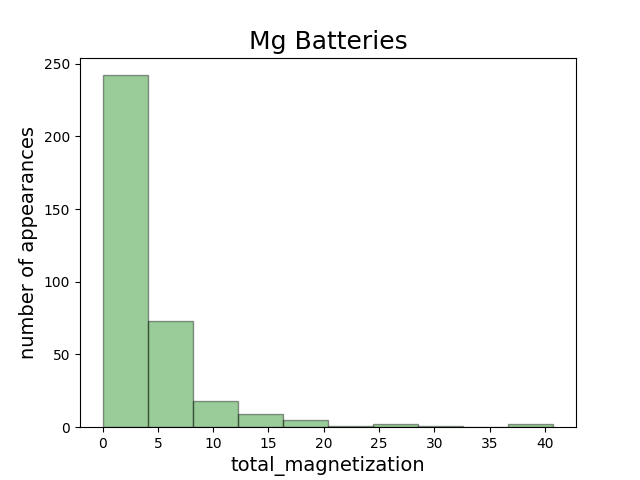
\includegraphics[width=\linewidth]{result/figures/distribution/Mg_distrof_total_magnetization.png}
         
     \end{subfigure}
          ~ 
     \begin{subfigure}{0.2\textwidth}
         \centering
         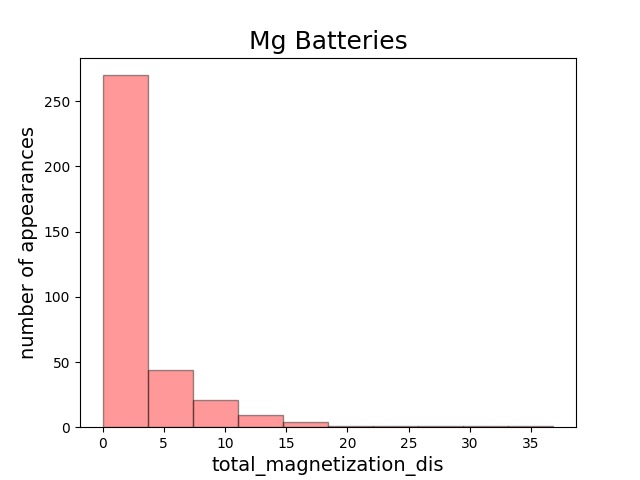
\includegraphics[width=\linewidth]{result/figures/distribution/Mg_distrof_total_magnetization_dis.png}
         
     \end{subfigure}
          ~ 
               \begin{subfigure}{0.2\textwidth}
         \centering
         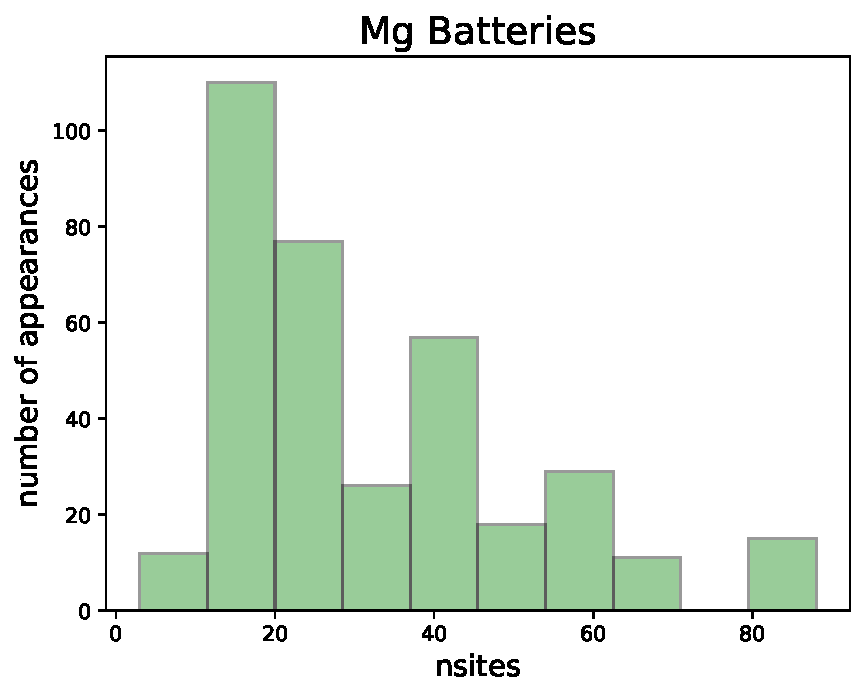
\includegraphics[width=\linewidth]{result/figures/distribution/columnsplotMg2_nsites.pdf}
         
     \end{subfigure}
          ~ 
     \begin{subfigure}{0.2\textwidth}
         \centering
         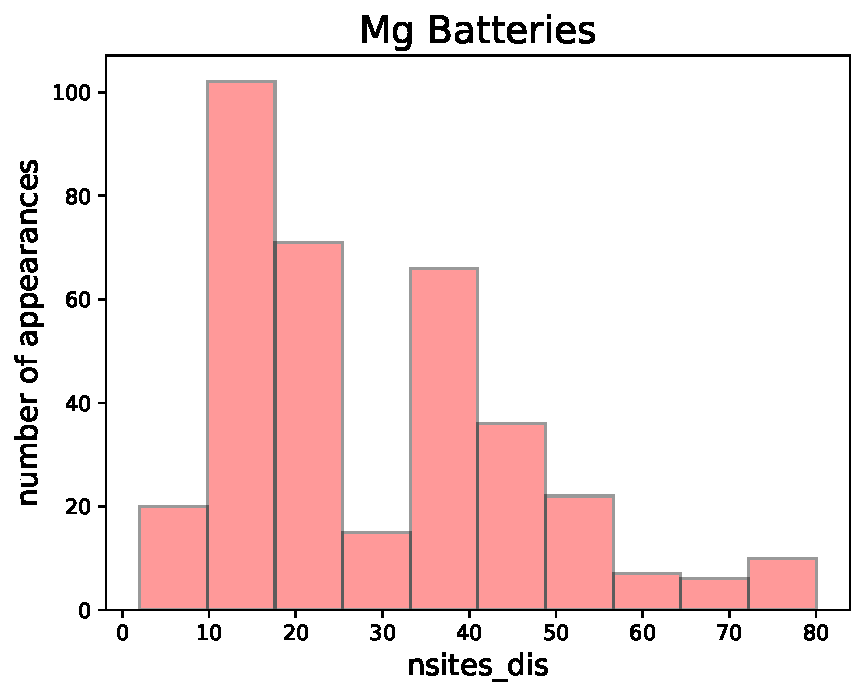
\includegraphics[width=\linewidth]{result/figures/distribution/columnsplotMg_nsites_dis.pdf}
         
     \end{subfigure}
                   ~ 
               \begin{subfigure}{0.2\textwidth}
         \centering
         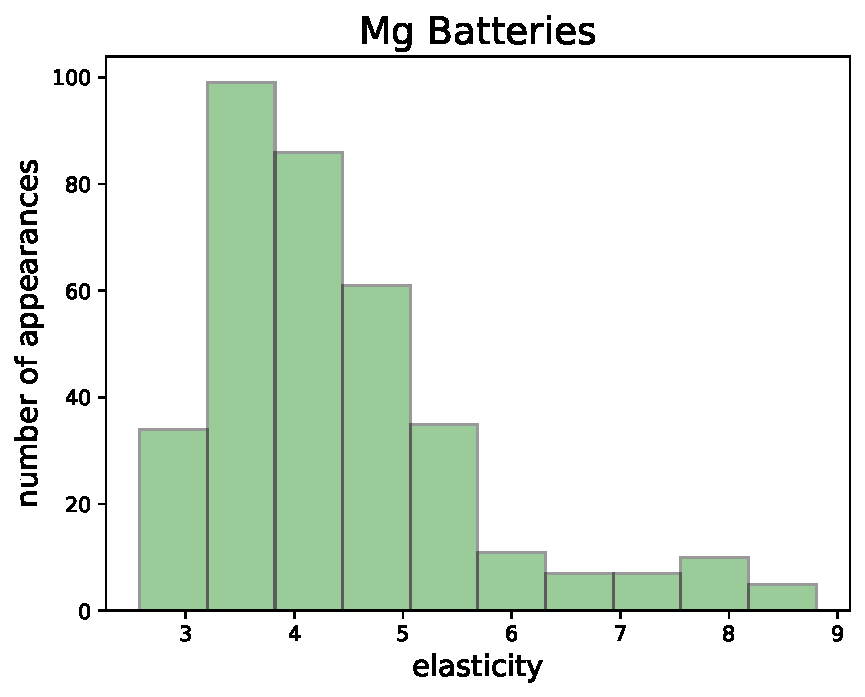
\includegraphics[width=\linewidth]{result/figures/distribution/columnsplotMg2_elasticity.pdf}
         
     \end{subfigure}
          ~ 
     \begin{subfigure}{0.2\textwidth}
         \centering
         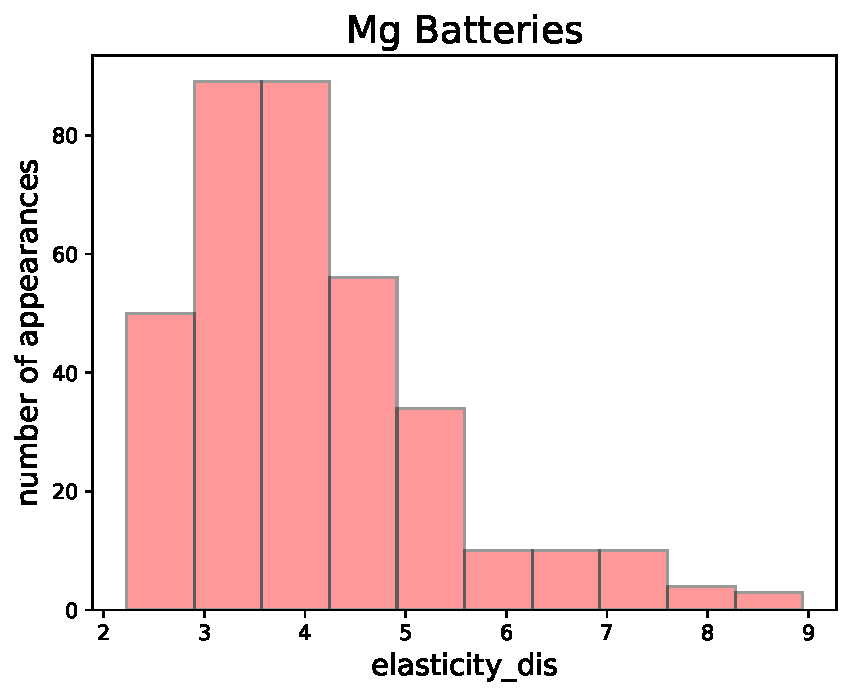
\includegraphics[width=\linewidth]{result/figures/distribution/columnsplotMg_elasticity_dis.pdf}
         
     \end{subfigure}
     \caption{These are the distributions of the $8$ material specific properties that account for the most variance, for both the \textcolor{green}{charged} and \textcolor{red}{discharged} material for the Mg-ion database. The x-axis are the feature values and the y-axis are the number of appearances for that range of feature values.}
     \label{fig:Mg_msp_distribution}
 \end{figure}
%--------------------------------------------------------------------------------
The results from the Mg-ion db, table \ref{tab:mg-msp}, shows that msp are correlated to the targets, with especially high values for AV ($60.9\%$). The accuracy for GC,VC, SE and ED are between $47.1-56.8 \%$, showing correlation for all targets and increasing error with the WAPE going from $7.9$ to $13.26\%$. The WAPE shows that the uncertainty is larger for SE and ED than for capacity and voltage. The $6-7$ features ignored by PCA are elasticity,  number of site, energy per atom, and the "charged volume". 

\begin{table}[h]
\normalsize
\title{Mg-db on msp}
\centering
\caption{msp prediction-scores for the Mg db tested against the given targets.}
\begin{tabular}{|c|c|c|c|c|c|}
	\hline 
	$\frac{Target: \rightarrow}{Accuracy:\downarrow} $ & AV & GC & VC & SE & ED 
	 \\ 
	\hline
	$R^2$-score & 0.5224 & 0.4023 & 0.47064 & 0.4997 &  0.4826\\ 
	\hline 
	$R^2$-train & 0.9293 & 0.9208 & 0.9078 & 0.9317 &  0.90721 \\ 
	\hline
	Mean: &2.5830	&194.105633	&844.3028&503.0492&2105.3873	\\
	\hline 
	Stdev:&0.2905	&22.8769	&103.3817	&79.9453	&399.8795	\\
	\hline
	RMSE:&0.2907& 22.9191& 103.3826 & 80.0723 & 400.4032 \\ 
	\hline 
	MAE: &0.2042& 16.7839 &  74.45455 & 61.0444 & 279.353 \\ 
	\hline
	WAPE: & 7.9079 & 8.6468 & 8.8184  & 12.1348	& 13.2685 \\
	\hline
	$R^2$-CVM:&  0.60989 & 0.471065 & 0.4985  & 0.56822 &0.5247 \\
	\hline
	components used: & 10/16 & 10/16 & 10/16  & 9/16 &9/16 \\
	\hline
\end{tabular}
\label{tab:mg-msp}
\end{table}

The results from the Mg-ion db, table \ref{tab:mg-msp}, shows that msp are correlated to the targets, with especially high values for AV ($60.9\%$). The accuracy for GC,VC, SE and ED are between $47.1-56.8 \%$, showing correlation for all targets and increasing error with the WAPE going from $7.9$ to $13.26\%$. The WAPE shows that the uncertainty is larger for SE and ED than for capacity and voltage. The $6-7$ features ignored by PCA are elasticity,  number of site, energy per atom, and the "charged volume". 

$R^2$-CVM on AV in the Li-ion db is lower than in the Mg-ion db, but the accuracy of the predictions are higher. GC and VC have a better score, but a larger error, while SE and ED have lower errors, and smaller scores. The components prioritized are the same as for the Mg-ion db, except for a couple of runs where it removes "charged density" as a predictor, which, for both runs, had a low variance ratio, meaning it had little variance compared with the other features.  

The increase in data seems to not effect our predictions to a large extent. $R^2$-train shows that our model is about as accurate on the data it has been presented. 
\FloatBarrier

\begin{table}[h]
\normalsize
\title{Li-db on msp}
\centering
\caption{msp from the Li-db tested against the given targets.}
\begin{tabular}{|c|c|c|c|c|c|}
	\hline 
	$\frac{Target: \rightarrow}{Accuracy:\downarrow} $ & AV & GC & VC & SE & ED  \\ 
	\hline
	$R^2$-score 	& 0.5384 & 0.4162 & 0.4870 & 0.3888 &  0.44016\\ 
	\hline 
	$R^2$-train 	&  0.9308 & 0.9146 & 0.9277 & 0.9189 & 0.9185 \\ 
	\hline
	Mean: 	 &3.58038&132.6524&463.5728&479.7717&1609.3506\\
	\hline 
	Stdev:	 &0.2853	&21.7816	&70.5023	&75.2707&272.7973	\\
	\hline
	RMSE: 	& 0.2853 & 21.804& 70.5346 & 75.323 & 735.50848 \\ 
	\hline 
	MAE: 	&0.1969& 15.3558 &  48.2923 & 55.3367 & 191.3195 \\ 
	\hline
	WAPE: 	& 5.5013 & 11.5759 & 10.4174  & 11.5339 & 11.8879 \\
	\hline
	$R^2$ CVM: &  0.5692 & 0.4456 & 0.5136  & 0.4572 & 0.4815 \\
	\hline
	components used: & 9/16 & 9/16 & 9/16  & 8/16 &9/16 \\
	\hline
\end{tabular}
\label{tab:Li-msp}
\end{table}

\subsubsection*{Stability}

In this work we tried to predict the stability of a material, based on the same predictors as introduced, this did not work. One possible reasons might be that this "stability" is connected to each particular material, it is not a property of the battery. Utilizing a combination of both charged and discharged properties to predict a feature related to only one of the two types of material can confuse the ML algorithm. The predictions on charged and discharged stability can be found on \href{https://github.com/sondrt/Machine-Learning-the-Voltage-Capacity-and-Energy-density-of-Electrode-Materials}{github}. In addition, we decided to include stability as a predictor to see if this upped our results. Using stability as a predictor did not increase the predictions over the threshold ($>2\%$) that was set. Yet, the ML model did include it in its predictions, so it contains relevant information and will therefor be kept.  
 


\FloatBarrier
\subsection{Volumetric number density}
\subsubsection*{Mg-ion framework}

\textbf{Volumetric number density} (vnd) as described (\ref{sec:volumetric_number_density}) are shown in table \ref{tab:mg-n-i},to \ref{tab:Li-vnd-iii}, first for the Mg-database then for the Li-database. Due to the nature of vnd, and our database having both charged and discharged materials, it is necessary to try the three alternatives; only the charged materials, only the discharged materials and the combination of both the charged and the discharged materials.

\begin{table}[h]
\normalsize
\centering
\caption{Mg- db, the charged material as vnd predictors. A total of 21 components are applicable. Mg-prediction results on the targets; Average Voltage (AV), gravimetric capacity (GV), volumetric capacity (VC), specific energy (SE), and energy density (ED). Each row showes the number representing that type of evaluation, as included in section (\ref{sec:evaluation_method}). } 
\title{Mg-db on n, charged materials}
\begin{tabular}{|c|c|c|c|c|c|}
	\hline 
	$\frac{Target: \rightarrow}{Accuracy:\downarrow} $ & AV & GC & VC & SE & ED 
	 \\ 
	\hline
	$R^2$-score 	& 0.51920 & 0.1783 	& 0.2513 & 0.5751 &   0.2864\\ 
	\hline 
	$R^2$-train 	& 0.94365 & 0.9055 	& 0.91827 & 0.9194 & 0.9302 \\ 
	\hline
	Mean: 		& 2.5492 &192.7605	&848.22	&537.5&2227.422\\
	\hline 
	Stdev: 		& 0.2604 &24.9649	&98.056&84.4191&335.7547\\
	\hline		
	RMSE:		 & 0.26043& 24.965 &  98.0653 &  84.5840 &336.2162 \\ 
	\hline
	MAE: 		& 0.1860 & 51.9769& 70.8905 & 63.5310 & 252.03396 \\ 
	\hline
	WAPE:		& 7.2986 & 9.2791 & 8.3575  & 11.8200 & 11.3150 \\
	\hline
	$R^2$ CVM: 	& 0.58126 &  0.2464 & 0.3964  & 0.5280 &0.5174 \\
	\hline
	components :	& 19/21 & 19/21 & 19/21  & 19/21 &19/21 \\
	\hline
\end{tabular}
\label{tab:mg-n-i}
\end{table}


\begin{table}[h]
\normalsize
\centering
\caption{Mg-db, the discharged material as vnd-predictors. A total of 30 components are applicable. Predictions on the targets; Average Voltage (AV), gravimetric capacity (GV), volumetric capacity (VC), specific energy (SE), and energy density (ED). Each row showes the number representing that type of test, as included in section (\ref{sec:evaluation_method}).}
\title{Mg database on n, the discharged materials}
\begin{tabular}{|c|c|c|c|c|c|}
	\hline 
	$\frac{Target: \rightarrow}{Accuracy:\downarrow} $ & AV & GC & VC & SE & ED 
	 \\ 
	\hline
	$R^2$-score 	& 0.4879 & 0.7213 & 0.5941 & 0.4612 &  0.4779\\ 
	\hline 
	$R^2$-train 	& 0.9312 &  0.92499 & 0.9332 & 0.9496 & 0.9218 \\ 
	\hline
	Mean: 	 	&2.7038	&184.0281&869.2605&483.4859& 2288.429	\\
	\hline 
	Stdev:		&0.2835	&24.0464	& 86.9195	&75.7915& 352.595	\\
	\hline		
	RMSE: 		&0.2836& 24.04749 &  86.9622 & 75.8086 & 352.6381 \\ 
	\hline
	MAE: 		& 0.1938 & 14.4620& 44.5180 & 57.4124 & 221.0466 \\ 
	\hline
	WAPE: 		& 7.1708 & 7.8586 & 5.1213  & 11.8746 & 9.6593 \\
	\hline
	$R^2$ CVM: 	& 0.5885 & 0.6190 & 0.64017  & 0.6115 &  0.5980 \\
	\hline
	components: 	& 22/30 & 22/30 & 22/30  & 22/30 &23/30 \\
	\hline
\end{tabular}
\label{tab:mg-n-ii}
\end{table}


\begin{table}[h]
\normalsize
\centering
\caption{Mg-db using both the discharged- and the charged materials as vnd-predictors. A total of 51 components are applicable. Predictions on the targets; Average Voltage (AV), gravimetric capacity (GV), volumetric capacity (VC), specific energy (SE), and energy density (ED). Each row showes the number representing that type of test, as included in section (\ref{sec:evaluation_method}).}
\title{Mg database on vnd, both charged and discharged}
\begin{tabular}{|c|c|c|c|c|c|}
	\hline 
	$\frac{Target: \rightarrow}{Accuracy:\downarrow} $ & AV & GC & VC & SE & ED 
	 \\ 
	\hline
	$R^2$-score 	& 0.6094 & 0.6150 & 0.7993 & 0.5685 &  0.6560\\ 
	\hline 
	$R^2$-train 	& 0.9507 & 0.9402 & 0.9452 & 0.9540 &  0.9385 \\ 
	\hline
	Mean: 	 	& 2.7871	&194.4788&825.5211&483.6478& 2166.943\\
	\hline 
	Stdev:	 	& 0.2405	&20.3516	&80.1226 	&69.5891	& 314.8012\\
	\hline 
	RMSE: 		&0.2409& 20.3608 &  80.1511 & 69.59 &314.8037\\ 
	\hline
	MAE: 		& 0.1857 & 11.9768& 38.6913 & 52.7039 & 219.9826 \\ 
	\hline
	WAPE: 		& 6.6656 & 6.1584 & 4.6868  & 10.8971 & 10.1517 \\
	\hline
	$R^2$ CVM: 	&  0.6261 	&  0.6622 	&  0.6758 	&  0.64942 & 0.6532 \\
	\hline
	components: 	& 30/51 	& 27/51 	& 29/51 	 & 29/51 	&27/51 \\
	\hline
\end{tabular}
\label{tab:mg-n-iii}
\end{table}


There are a couple of different results that are particularly interesting. First of all; The use of all vnd-predictors yield the best predictions in all cases, with the lowest error in almost all. When combining the two group of predictors PCA tells us that there is an overlap in the information from the charged and discharged materials as given by the number of components used by the ML algorithm. \textit{i.e.} for charged materials $19/21$ components where used to account for $99\%$ of the variance in the data, for the discharged materials $22/30$ components where used, while when combined $30$ out of the total $51$ components were necessary to achieve the same $99\%$. This shows an overlap in the two group of predictors data.

	There are targets that respond better to the use of one state of material, charged or discharged, than the other. Gravimetric and volumetric capacity responds particularly well to the discharged materials with a $R^2$-CVM $= 0.6226$, but improve (by a small percentage $3-5\%$) when given the combination of materials, and the error decreases. AV is the only target that has the same prediction for both charged and discharged, but it is a clear improvement when combining both with an increase in $R^2$-CVM of around $4\%$. This seems reasonable due to the discharged materials containing more information because of the discharged material set having a larger number of atom types, and that atom (Mg) being the only atom all batteries have in common (i.e. the battery framework $\ce{Mg_{0-1}CrF_6}$ with $\ce{CrF_6}$ being the charged material and  $\ce{MgCrF_6}$ being the discharged material).


When combining the two group of predictors our predictions on all five targets are between $62$ to $68$ percent, with high certainty. Which showes that this is a good predictor for all of these targets. Noticeably the $R^2$-train is also considerably better both for the combination of materials and for the msp.  


Lastly, the quality of our estimator is significantly lower for specific energy and energy density. It seems that the quality of our predictor drops on these predictors. (SP $- \si{Wh/kg}$, ED $- \si{Wh/l}$). \myworries{why? whywhywhy?}

\FloatBarrier
\subsubsection*{Predictions on Li-ion intercalation frameworks with vnd}
The same technique, as used in the previous section, was applied to the Li-ion db, with $2108$ battery frameworks instead of $365$, as were the case for Mg-ion intercalation type db. The Li-ion db is a bigger database with different and more unique atom types, which is likely to calls for more variability, possibly more bias, and most likely a lower uncertainty in the predictions.

First of all, it is no obvious improvement when using only the discharged materials, over only the charged materials, as were with the Mg-ion db. 

If we combining the two, we quickly see that the variation in the data behaves in the same way as for the Mg db, there is an obvious overlap in information and correlation in the predictors. Volumetric capacity, with the overall best predictions ($71.86\%$), only uses $38$ components, out of the possible $107$ (to account for $99\%$ of the variance). When using the charged and discharged predictors the machine learning algorithm used $38/54$ components for the charged material and $34/53$ components for the discharged components. It stands to reason that volumetric capacity would be a good target for vnd due to the intrinsic relation to volume. Because of this, it stands to reason that it should be a better predictor for ED than for SE, as it is, with an increase of $9\%$. The features that PCA removes are the atom types with rare occurrences, these features mostly contain zeroes, and if they contain other values they are hard to make relevant decision rules from.  

Average voltage predictions are $56\%$ with high certainty, lower than the predictions for the Mg-ion db, but a bit higher accuracy. The AV lacks a obvious connection to the atom types in them selvs and volume. Therefore one can hypothesis that it will get better when combined with a representation of energy from the msp or electronegativity through AP-RDF.



\begin{table}[h]
\normalsize
\title{Li-db on vnd - charged}
\centering
\caption{Li - vnd charged.}
\begin{tabular}{|c|c|c|c|c|c|}
	\hline 
	$\frac{Target: \rightarrow}{Accuracy:\downarrow} $ & AV & GC & VC & SE & ED 
	 \\ 
	\hline
	$R^2$-score 	& 0.4466 & 0.22431 & 0.4248 	&  0.40232 &  0.3402\\ 
	\hline 
	$R^2$-train 	& 0.9321 & 0.9060 	& 0.9170 	& 0.9166 	& 0.9287 \\ 
	\hline
	Mean: 		&3.589	&134.03	&467.40	&480.46	&1628.3	\\
	\hline 
	Stdev:		&0.2884	&22.165	&73.304	&75.481	&241.6	\\
	\hline
	RMSE: 		& 0.2888 & 22.174	& 73.313 	& 75.538	 & 241.8 \\ 
	\hline 
	MAE: 		& 0.1952 & 15.371	 & 49.472	 & 53.076	 & 176.38 \\ 
	\hline
	WAPE: 		& 5.440 	&  11.469 	& 10.584  	& 11.047 	&10.833 \\
	\hline
	$R^2$ CVM: 	& 0.5437 & 0.3692 	& 0.4352  	& 0.4324 	&0.4690 \\
	\hline
	components used: & 37/54 & 41/54 & 38/54  & 38/54 &35/54 \\
	\hline
\end{tabular}
\label{tab:Li-vnd-i}
\end{table}

\begin{table}[h]
\normalsize
\title{Li-db on vnd - discharged}
\centering
\caption{Li- vnd discharged.}
\begin{tabular}{|c|c|c|c|c|c|}
	\hline 
	$\frac{Target: \rightarrow}{Accuracy:\downarrow} $ & AV & GC & VC & SE & ED 
	 \\ 
	\hline
	$R^2$-score 	& 0.5099 &  0.3731 & 0.4539 & 0.3133 &  0.3519\\ 
	\hline 
	$R^2$-train  	 & 0.9269 & 0.9163 & 0.9248 & 0.9178 & 0.9122 \\ 
	\hline
	Mean:	 	 &3.5455	& 133.12&476.6359&473.7458	&1609.5469\\
	\hline 
	Stdev:		 &0.2858	&21.237&70.9524&76.4492&292.0871\\
	\hline
	RMSE:		 & 0.2860 & 21.2419& 70.95331 & 76.4636 & 292.1071 \\ 
	\hline 
	MAE:	 	&0.1895& 14.1890 &  45.2840 & 54.9314 & 177.8518 \\ 
	\hline
	WAPE: 		& 5.3454 & 10.659 & 9.501  & 11.5951 &11.0498 \\
	\hline
	$R^2$ CVM: &  0.5319 & 0.3983 & 0.4724  &  0.4367 &0.44020 \\
	\hline
	components used: & 40/53 &  38/53 &  34/53  &  39/53 & 39/53 \\
	\hline
\end{tabular}
\label{tab:Li-vnd-ii}
\end{table}

\begin{table}[h]
\normalsize
\title{Li-db on vnd - charged and discharged}
\centering
\caption{Li- vnd both charged and discharged}
\begin{tabular}{|c|c|c|c|c|c|}
	\hline 
	$\frac{Target: \rightarrow}{Accuracy:\downarrow} $ & AV & GC & VC & SE & ED 
	 \\ 
	\hline
	$R^2$-score 	& 0.4755 & 0.54190 & 0.6923 & 0.5388 &  0.5912\\ 
	\hline 
	$R^2$-train 	& 0.9355 & 0.94517 & 0.9550 &   0.9351 & 0.9476 \\ 
	\hline
	Mean: 		&3.616	&135.22&460.05&473.75	&1643.15	\\
	\hline 
	Stdev:	 	&0.2657	&17.383	&54.816	&69.721	&213.12	\\
	\hline
	RMSE: 		& 0.2661 & 17.390	& 54.830 & 69.779	 & 213.17 \\ 
	\hline 
	MAE: 		&0.1859& 11.089	 &  32.248 & 46.392 & 144.95 \\ 
	\hline
	WAPE: 		& 5.141 & 8.201 	&  7.0095  & 9.793 &8.822 \\
	\hline
	$R^2$ CVM: 	&  0.5608 & 0.6191 & 0.7186  & 0.5619 &0.6506 \\
	\hline
	components used: & 39/107 & 37/107 & 38/107  & 38/107 &40/107 \\
	\hline
\end{tabular}
\label{tab:Li-vnd-iii}
\end{table}






%$n$ is overall better at predicting VC and with that GC naturally follows. In the first figure(\ref{tab:mg-n}), the Mg-database, every prediction has a lower 'score' than in the Li-database. This is probably due to it being a much smaller database. 

%\myworries{Should do better calculations on this, maybe when results and Battery-section is done.}

%As can be seen clearly; the evaluations of this method is somewhat splitt. The MSE is generally better for the Li-database, and is best at the AV. The CV is better for the capacities but there is somewhat a high degree of uncertainty. This is probably due to the database being small. As expected the results for volumetric capacity is the peak of these runs. 

%One can from these results conclude that volumetric number density is worth bringing on as a predictor, as it clearly is a part of the puzle.  




\FloatBarrier
\subsection{Void fraction}
Results for predictions using only the \textbf{void fraction} (\ac{vf}) methods predictors, that is, the charged and discharged materials, helium volume and geometric volume. First on the Mg-ion db, then on the Li-ion db.

	On its role as a predictor, the void fraction could be a good predictor, both from its success on predictions of other type of materials and the changes that occur in the space occupied by the ion in the discharged material against the charged material. We will first have a look at the distribution of the features set. 

\subsubsection{Distribution}
%\subsubsection*{Predictions on Mg-ion intercalation frameworks with the void fraction predictors}

 \begin{figure}[h]
     \centering
     \begin{subfigure}{0.23\textwidth}
         \centering
         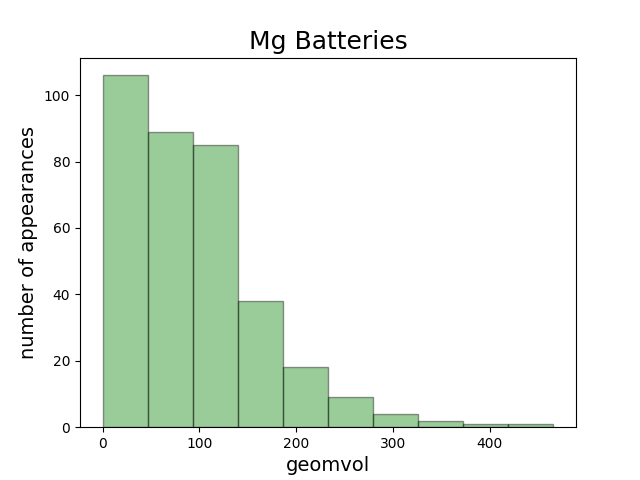
\includegraphics[width=\linewidth]{result/figures/distribution/Mg_distrof_geomvol.png}
     \end{subfigure}
     ~ 
     \begin{subfigure}{0.23\textwidth}
         \centering
         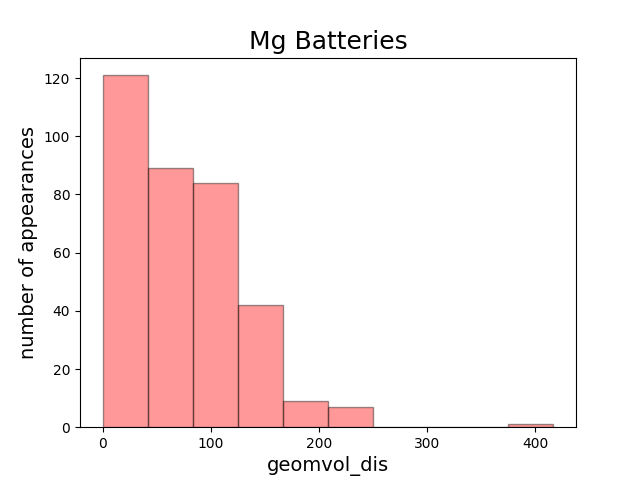
\includegraphics[width=\linewidth]{result/figures/distribution/Mg_distrof_geomvol_dis.png}
     \end{subfigure}
          ~ 
     \begin{subfigure}{0.23\textwidth}
         \centering
         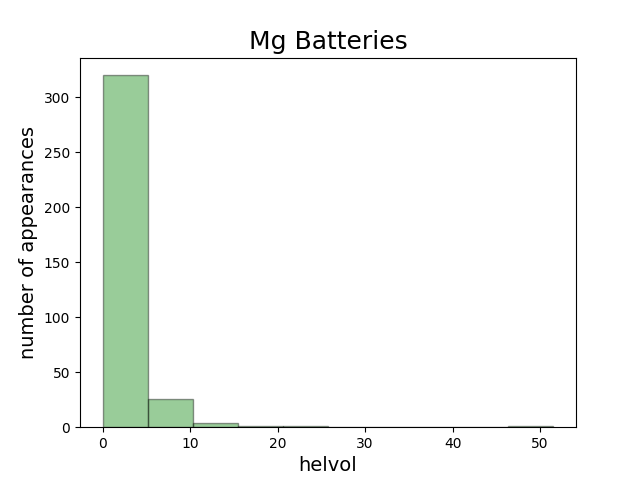
\includegraphics[width=\linewidth]{result/figures/distribution/Mg_distrof_helvol.png}
     \end{subfigure}
          ~ 
     \begin{subfigure}{0.23\textwidth}
         \centering
         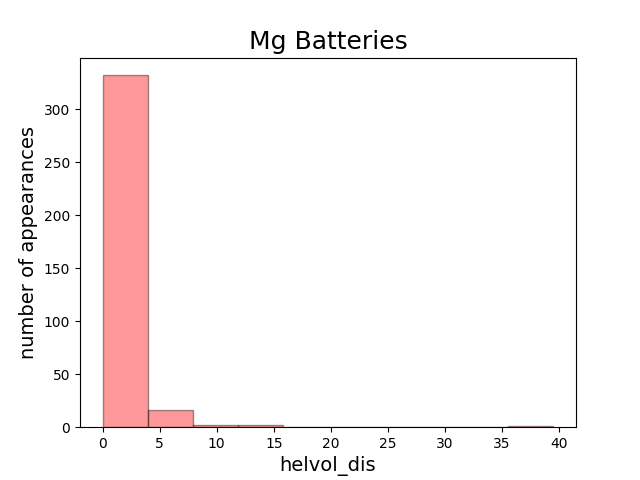
\includegraphics[width=\linewidth]{result/figures/distribution/Mg_distrof_helvol_dis.png}
     \end{subfigure}
\caption{Distribution of the void fraction predictors, geometric volume and helium volume, as calculated by Poreblazer for the Mg-ion db. \textcolor{teal}{Charged} features in green and \textcolor{red}{discharged} features in red}
\label{fig:Mg_distri_VF}
\end{figure}

 \begin{figure}[h]
     \centering
     \begin{subfigure}{0.23\textwidth}
         \centering
         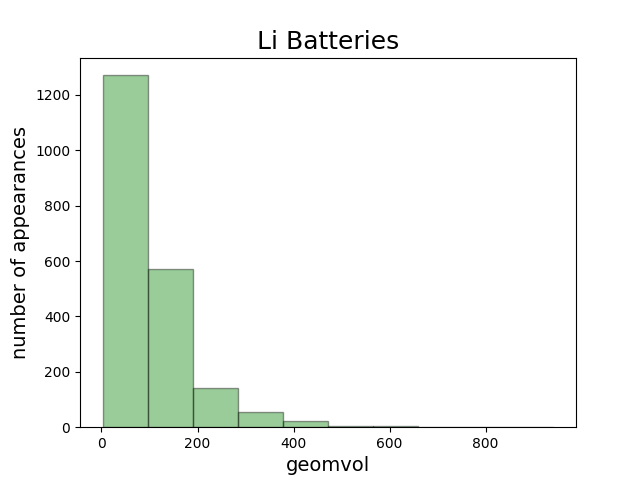
\includegraphics[width=\linewidth]{result/figures/distribution/Li_distrof_geomvol.png}
     \end{subfigure}
     ~ 
     \begin{subfigure}{0.23\textwidth}
         \centering
         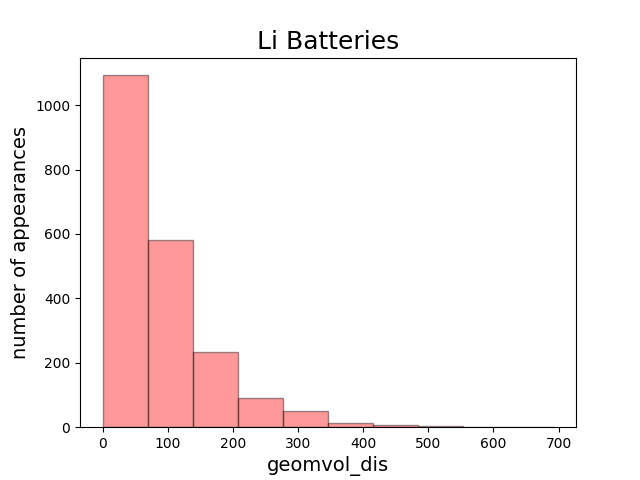
\includegraphics[width=\linewidth]{result/figures/distribution/Li_distrof_geomvol_dis.png}
     \end{subfigure}
          ~ 
     \begin{subfigure}{0.23\textwidth}
         \centering
         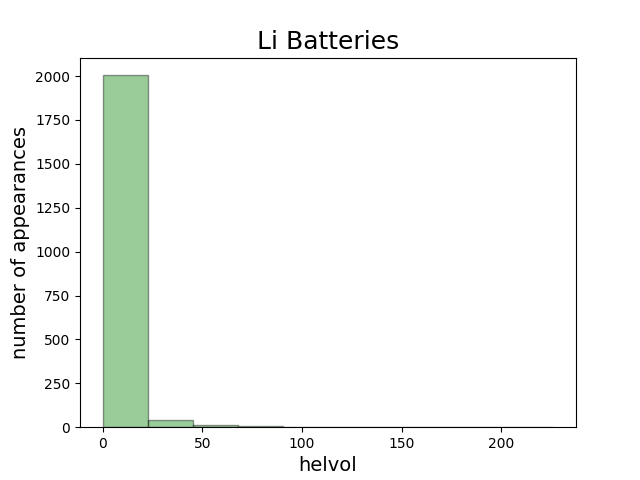
\includegraphics[width=\linewidth]{result/figures/distribution/Li_distrof_helvol.png}
     \end{subfigure}
          ~ 
     \begin{subfigure}{0.23\textwidth}
         \centering
         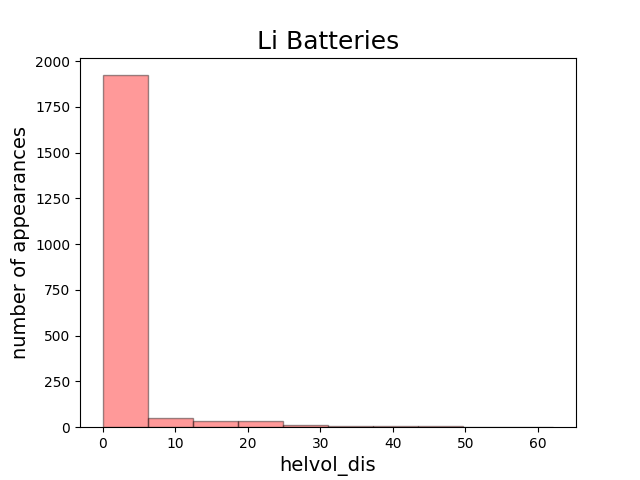
\includegraphics[width=\linewidth]{result/figures/distribution/Li_distrof_helvol_dis.png}
     \end{subfigure}
\caption{Distribution of the void fraction predictors, geometric volume and helium volume, as calculated by Poreblazer for the Li-ion db.}
\label{fig:Li_distri_VF}
\end{figure}


\subsubsection{Predictions}


The results for vf as a predictor for the Mg-ion db is shown in table \ref{tab:mg_vg}. Void fraction seems to be inaccurate for most targets, with the best accuracy score of $39.4\%$ on volumetric capacity. Second best prediction is on gravimetric capacity ($34.9\%$), which is closly related. The other predictions have to low correlation to consider them as predictors, so AV, SE and ED will be omitted for the rest of this subsection.

\begin{table}[h]
\normalsize
\centering
\caption{Mg- db prediction on the targets AV, GC, VC, SE, ED. A total of 4 predictors where used in this run.}
\title{Mg database on voidfraction}
\begin{tabular}{|c|c|c|c|c|c|}
	\hline 
	$\frac{Target: \rightarrow}{Accuracy:\downarrow} $ & AV & GC & VC & SE & ED 
	 \\ 
	\hline
	$R^2$-score & -0.3240 & 0.2858 & 0.2387 & 0.12553 &  0.06999\\ 
	\hline 
	$R^2$-train & 0.8621 &  0.9047 & 0.9266 & 0.8821 & 0.89021 \\ 
	\hline
	Mean: 	& 2.657	&185.0915&830.5563& 492.9507	&2181.7746\\
	\hline 
	Stdev:	&0.4195	&27.3274	&93.0447&111.29816	&420.6466\\
	\hline 
	RMSE:	 &0.4197& 27.3296 &  93.07669 & 111.3178 & 420.6466 \\ 
	\hline
	MAE: 	& 0.3229 & 19.6535& 68.1477 & 88.04975 & 324.1471 \\ 
	\hline
	WAPE: 	& 12.1522 & 10.6182 & 8.20506  & 17.8617 & 14.85704 \\
	\hline
	$R^2$ CVM: & 0.06214 &  0.3490 & 0.3943  & 0.09092 & 0.18253 \\
	\hline
	components: & 3/4 	& 4/4 	& 4/4 	 & 3/4	 & 3/4 \\
	\hline
\end{tabular}
\label{tab:mg_vg}
\end{table}



%\subsubsection*{Predictions on Li-ion intercalation frameworks with the void fraction predictors}

On the Li-ion db (presented in table \ref{tab:Li-vf}) the same trend as on Mg-ion db seems persistent. More data seems to emphasize that the void fraction is not a inadequate descriptor for the given targets. The best predictions are still on VC with $15\%$ accuracy, followed by GC  with $5\%$ accuracy, but the scores being this low, and  . 

\begin{table}[h]
\normalsize
\centering
\caption{Li- db prediction on the targets AV, GC, VC, SE, ED. A total of 4 predictors where used in this run.}
\title{Li database on void fraction}
\begin{tabular}{|c|c|c|c|c|c|}
	\hline 
	$\frac{Target: \rightarrow}{Accuracy:\downarrow} $ & AV & GC & VC & SE & ED 
	 \\ 
	\hline
	$R^2$-score 	& -0.0373 & 0.0603 & 0.05857 &  -0.1374 &  0.01655\\ 
	\hline 
	$R^2$-train 	&  0.8510 &  0.87095 & 0.89077 &  0.8601 & 0.8669 \\ 
	\hline
	Mean: 		 &3.5262&133.9714&447.216	&457.3083&1636.7998	\\
	\hline 
	Stdev:		 &0.3914	&26.2527	&90.6257&102.7326&345.827\\
	\hline 
	RMSE: 		&0.0455& 26.253 &  90.6261 & 102.74241 & 345.8724 \\ 
	\hline
	MAE: 		& 0.3028 & 19.6381& 66.8044 & 76.8657 & 261.30785 \\ 
	\hline
	WAPE: 		& 8.5886 & 14.6584 & 14.9378  & 16.8082 & 15.9645 \\
	\hline
	$R^2$ CVM: & -0.06318 & 0.05186 & 0.159419  & -0.02663 & 0.02518 \\
	\hline
	components: & 3/4 	& 4/4 & 4/4  & 4/4 & 4/4 \\
	\hline
\end{tabular}
\label{tab:Li-vf}
\end{table}


In all runs, three to four feature were needed to account for $99\%$ of the variability. Between $80-90\%$ of the variability can be traced back to one predictor, namely geometric volume for the discharged materials, and yet it is only possible to get a $R^2$-CVM prediction above $0\%$ for any target, by including all 4 predictors. This points at void fraction, as we have approached it here, being a bad descriptor for the given targets. 

It seems reasonable that $90\%$ of the variability are in one predictor due to these 4 predictors measuring the same physical , this physical feature seems to be expressed by having some correlation with the volumetric capacity, but this correlation might be covered by noise as we introduce more data.

Void fraction was tested as a predictor for VC, and other targets, in combination with other predictors, but due to drops in predictive capability the results are omitted from the result section. These results can be found on github.
%It is clear that our ML model is missing vital information to make better prediction, due to $R^2$-train score being low. $R^2$-train should approach $100\%$ if there are enough correlation in the data, we have not limited the depth of our trees, so if possible, the ML model will try to make full branches from root to leaf node, which means that it would memorize the answers because the data is already known to the ML algorithm. It might also show that our data contains to much noise, which does not seem very likely, because of our strictly defined predictors. 

%----------------------------------------------------------------------------
\FloatBarrier
\subsection{Atomic property weighted radial distribution function}
\subsubsection{Row approach to AP-RDF }%------------------------------------

The second approach gave correlation with the targets as presented in table \ref{tab:Mg-APRDF2} for the Mg-ion db and in table \ref{tab:Li-APRDF2} for the Li-ion db, here we added a new columns per value from the RDF, as explained in the section \ref{sec:APRDF}. 

This approach seems promising with scores that indicates correlation for all targets, that increases on AV and ED for the Li-ion. The WAPE decreases for AV and SE but increases for GC and VC, for a larger db witch indicates. The correlation is stable when we switch to the Li-ion db, which indicates that we have represented a property in a reasonable fashion. The second approach to AP-RDF will be discussed in more detail when the combined predictions are presented.  


\begin{table}[h]
\normalsize
\centering
\caption{Mg- db prediction on the targets AV, GC, VC, SE, ED.  A total of 106 components are applicable. A total of  predictors where used in this run.}
\title{Mg database on void fraction}
\begin{tabular}{|c|c|c|c|c|c|}
	\hline 
	$\frac{Target: \rightarrow}{Accuracy:\downarrow} $ & AV & GC & VC & SE & ED 
	 \\ 
	\hline
	$R^2$-score & 0.1793 & 0.3855 & 0.3334 &  0.3711 &  0.3206\\ 
	\hline 
	$R^2$-train & 0.8741 &  0.8986 & 0.92503&  0.88771 & 0.8978 \\ 
	\hline
	Mean: 	&2.7054	&200.669&836.204	&519.0915&2250.88	\\
	\hline 
	Stdev: 	&0.4042	&25.4534	&89.270	&103.0931&395.374	\\
	\hline 
	RMSE: &0.4041& 25.464 &  89.3011 & 103.19 & 395.53 \\ 
	\hline
	MAE: & 0.3163 & 18.420& 63.552 &  77.924 & 290.96 \\ 
	\hline
	WAPE: &  11.6913 & 9.1792 & 7.6001  & 15.0115 & 12.9264 \\
	\hline
	$R^2$ CVM: & 0.2336 & 0.3956 &  0.4438  & 0.3611 & 0.32963 \\
	\hline
	components: & 18/106 & 46/106 & 35/106  & 17/106 & 35/106 \\
	\hline
\end{tabular}
\label{tab:Mg-APRDF2}
\end{table}

\begin{table}[h]
\normalsize
\centering
\caption{Li db prediction on the targets AV, GC, VC, SE, ED. A total of 106 components are applicable. A total of  predictors where used in this run.}
\title{Li database on void fraction}
\begin{tabular}{|c|c|c|c|c|c|}
	\hline 
	$\frac{Target: \rightarrow}{Accuracy:\downarrow} $ & AV & GC & VC & SE & ED 
	 \\ 
	\hline
	$R^2$-score & 0.2894 & 0.2732 & 0.4094 &  0.2666 &  0.3280\\ 
	\hline 
	$R^2$-train & 0.8951 &  0.9032 & 0.9191 &  0.9003 & 0.9043 \\ 
	\hline
	Mean: &3.4851	&134.104	&460.5513&476.3011&1590.0499\\
	\hline 
	Stdev:&0.3428&22.71	&74.7006	&85.6635	&295.106	\\
	\hline 
	RMSE: &0.2503& 22.7127 &  74.706 & 85.6724 & 295.1143 \\ 
	\hline
	MAE: & 0.6937 & 15.74474& 52.9488 &  61.4651 & 202.1444 \\ 
	\hline
	WAPE: & 7.1808 & 11.7406 & 11.4968  & 12.90 & 12.7131 \\
	\hline
	$R^2$ CVM: & 0.3075 & 0.3379 & 0.4474  & 0.3502 & 0.3771 \\
	\hline
	components: & 42/106 & 46/106 & 44/106  & 46/106 & 46/106 \\
	\hline
\end{tabular}
\label{tab:Li-APRDF2}
\end{table}

\subsubsection{Cross-product approach}
The AP-RDF was tested with a cross-product approach, this is explained in the method section \ref{sec:APRDF}. As is clear from the tables \ref{tab:Mg-APRDF1} the first approach to AP-RDF did not give a good correlation with the targets and the error is to big, and will not be considered further. The idea was that it is better for a RF approach to consider longer trees rather than more features. These results are still of interest in a ML perspective. When combined with other predictors it was clear that the ML model learned memorized what results belonged to what predictors. It could do this because of how the test data was randomly split, not accounting for target duplicates, but when tested with only the 7 features belonging to this AP-RDF approach it did not manage to memorizing the data. Pointing at it not being enough correlation in the data to find a solid pattern. The cross-product approach will not be considered further, and due to the size of such calculations the Li-ion db was also omitted from testing.
 

\begin{table}[htbp]
\normalsize
\centering
\caption{Mg db prediction on the targets AV, GC, VC, SE, ED. A total of 6 predictors where used in this run; radius, electronegative, van der waals volume and polarization, all for both charged and discharged materials. }
\title{Mg database on AP-RDF}
\begin{tabular}{|c|c|c|c|c|c|}
	\hline 
	$\frac{Target: \rightarrow}{Accuracy:\downarrow} $ & AV & GC & VC & SE & ED 
	 \\ 	\hline
	$R^2$-score &  0.0284 & 0.0799 & 0.1116 &  0.0323 &  0.0540\\  \hline 
	$R^2$-train & 0.40632 &   0.37274 & 0.3877 &  0.3927 & 0.3998 \\ \hline
	Mean: & 2.6294&196.4378&826.694	&509.643	& 2120.2996	\\ \hline 
	Stdev: &0.8531	&69.896	&279.4123&244.658	&990.4840	\\ \hline 
	RMSE: &1.1041& 85.8334 &  279.413 &  244.6616 & 990.4908 \\ \hline
	MAE: & 0.637 & 47.4149& 192.349 &  175.8229 & 703.5917 \\  \hline
	WAPE: & 24.2602 & 24.1374 & 23.267  & 34.4992 & 33.1835 \\ \hline
	$R^2$ CVM: &  0.0309 & 0.11039 & 0.13321 & 0.04783 & 0.05931 \\	 \hline
	components: & 6/6 & 6/6  & 5/6   & 6/6 & 6/6  \\ 	\hline
\end{tabular}
\label{tab:Mg-APRDF1}
\end{table}

    

\FloatBarrier
\subsection{Combining predictors} 
In this subsection predictors combined. The combination of msp and vnd are of particular interest and will therefore get special attention 
 table \ref{tab:mg-vnd-msp} and \ref{tab:Li-vnd-msp}, the predictors: msp and vnd, were combined. The Mg-ion db predictions increase for AV and SE ($3\%$, $7\%$ ), while it stays still for GC, VC and ED (change $ < 2\%$). The WAPE falls which indicates that the predictions are more reliable.

The combining msp and vnd, for the Li-ion db, the trends are consistent with the Mg-ion db. For AV and SE the predictions increases ($13\%$, and $11\%$) and WAPE goes down. For the predictions in general, the combination of predictors either heightens the predictive score, lowers the error or both. 
 
\begin{table}[h]
\normalsize
\centering
\caption{Mg-db applying msp and vnd. A total of 66 components are applicable. Predictions on the targets; Average Voltage (AV), gravimetric capacity (GV), volumetric capacity (VC), specific energy (SE), and energy density (ED). Each row showes the number representing that type of test, as included in section (\ref{sec:evaluation_method}).}
\title{Mg database on vnd and msp}
\begin{tabular}{|c|c|c|c|c|c|}
	\hline 
	$\frac{Target: \rightarrow}{Accuracy:\downarrow} $ & AV & GC & VC & SE & ED 
	 \\ 
	\hline
	$R^2$-score 	& 0.6205 & 0.5940 & 0.66789 & 0.6710 &  0.5324\\ 
	\hline 
	$R^2$-train 	& 0.9445 & 0.9512 & 0.9611 & 0.94143 &  0.9334 \\ 
	\hline
	Mean: 	 	& 2.6786	&194.662&828.9436& 548.585& 2142.81\\
	\hline 
	Stdev:	 	& 0.2612	&18.9257	&67.7563 	&68.168	& 341.56\\
	\hline 
	RMSE: 		&0.2612& 18.9269 &  67.7746 & 68.1804 &341.58\\ 
	\hline
	MAE: 		& 0.1881 & 10.8578& 34.5623 & 49.1891 & 219.49 \\ 
	\hline
	WAPE: 		& 7.0254 & 5.57778 & 4.1694  & 8.9665 & 10.2428 \\
	\hline
	$R^2$ CVM: 	& 0.6618 	& 0.6661 	& 0.6930	& 0.7209&0.6424 \\
	\hline
	components: 	& 34/66 	& 35/66 	& 35/66 	 & 33/66 	&34/66 \\
	\hline
\end{tabular}
\label{tab:mg-vnd-msp}
\end{table}

\begin{table}[h]
\normalsize
\centering
\caption{Li-db applying msp and vnd. A total of 123 components are applicable. Predictions on the targets; Average Voltage (AV), gravimetric capacity (GV), volumetric capacity (VC), specific energy (SE), and energy density (ED). Each row showes the number representing that type of test, as included in section (\ref{sec:evaluation_method}).}
\title{Li database on vnd and msp}
\begin{tabular}{|c|c|c|c|c|c|}
	\hline 
	$\frac{Target: \rightarrow}{Accuracy:\downarrow} $ & AV & GC & VC & SE & ED 
	 \\ 
	\hline
	$R^2$-score 	& 0.5721 & 0.6090 & 0.6824 & 0.66525 &  0.6344\\ 
	\hline 
	$R^2$-train 	& 0.9609 & 0.9533 & 0.9574 & 0.9455 &  0.9528 \\ 
	\hline
	Mean: 	 	& 3.6302	&131.3345&467.1239& 471.7594& 1664.6278\\
	\hline 
	Stdev:	 	& 0.2022	&15.6615	&54.1556 	&62.4251	& 196.7591\\
	\hline 
	RMSE: 		&0.20225& 15.6676 &  54.16726 & 62.4668 &196.8365\\ 
	\hline
	MAE: 		& 0.1474 & 10.8578& 34.45520 & 41.13432 & 135.256 \\ 
	\hline
	WAPE: 		& 4.0622 & 7.86381 & 7.37602  & 8.7193 & 8.1252 \\
	\hline
	$R^2$ CVM: 	& 0.6979 	& 0.6444 	& 0.71029 & 0.6713 &0.6590 \\
	\hline
	components: 	& 43/123 	& 44/123 	& 45/123 	 & 46/123 	&45/123 \\
	\hline
\end{tabular}
\label{tab:Li-vnd-msp}
\end{table}

Figure \ref{fig:predontarg_Mg} and \ref{fig:predontarg_Li} summarizes the $R^2$-CVM for all targets, over the predictors presented. The utmost right labeled "combo" is the combination of the predictors msp (with stability), void fraction and vnd. "APRDF1" are not included in figure \ref{fig:predontarg_Li} as stated earlier. 

 \begin{figure}[h]
    \centering
    \begin{subfigure}{1\textwidth}
        \centering
        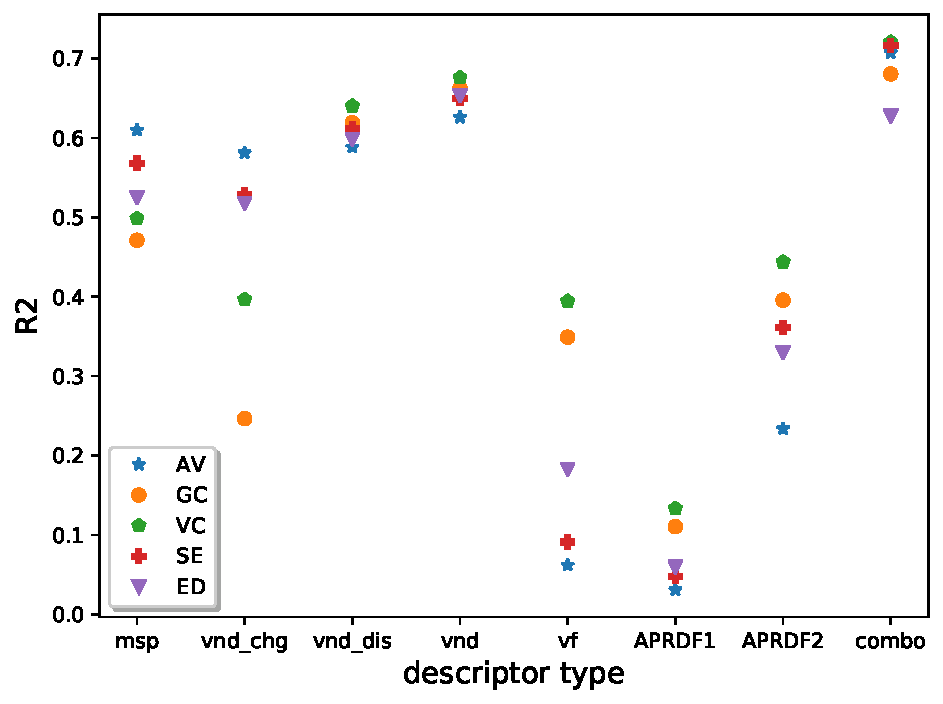
\includegraphics[width=\linewidth]{result/figures/Mg_pred_on_targ.pdf}
    \end{subfigure}
        \caption{Mg}
        \label{fig:predontarg_Mg}
\end{figure}    

\begin{figure}[h]
    \centering
  \begin{subfigure}{1\textwidth}
        \centering
        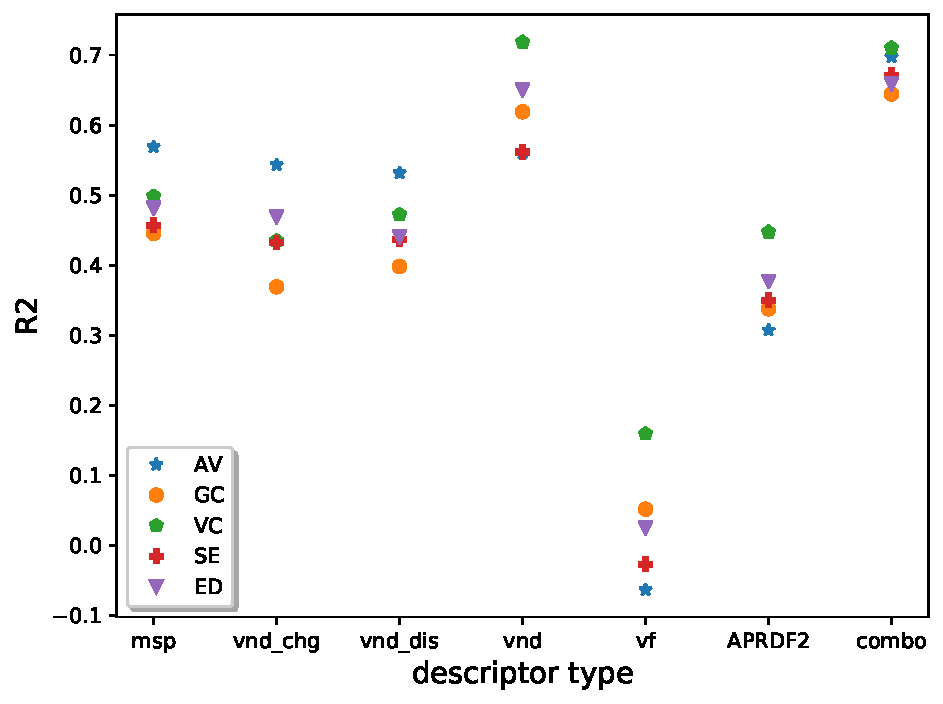
\includegraphics[width=\linewidth]{result/figures/Li_pred_on_targ.pdf}
    \end{subfigure}%
        \caption{Li}
        \label{fig:predontarg_Li}
\end{figure}

\FloatBarrier
\subsubsection{Combining predictors and targets}


In a last effort to evaluate the method some of the targets were introduced as predictors. The idea being is that if one of the targets is simple to compute, with \textit{e.g.} DFT, then it is possible to predict the other targets without preforming costly calculations. In essence a way to speed up high-throughput material science. First the Mg-ion db will be considered, then the Li-ion db and at the end a combination of different targets will briefly be looked at. 

%I.e. by introducing the voltage as a predictors for specific energy and energy density the predictions does a jump to above $80\%$. 

\begin{table}[h]%Mg msp,vnd,stab,vf
\normalsize
\centering
\caption{Mg-db applying msp, vnd, stability and void fraction. A total of 72 components are applicable. Predictions on the targets; Average Voltage (AV), gravimetric capacity (GV), volumetric capacity (VC), specific energy (SE), and energy density (ED). Each row shows the number representing that type of test, as included in section (\ref{sec:evaluation_method}).}
\title{Mg database on vnd, msp, vf and stability}
\begin{tabular}{|c|c|c|c|c|c|}
	\hline 
	$\frac{Target: \rightarrow}{Accuracy:\downarrow} $ & AV & GC & VC & SE & ED 
	 \\ 
	\hline
	$R^2$-score 	& 0.6748 & 0.6743 & 0.6952 & 0.6786 &  0.5836\\ 
	\hline 
	$R^2$-train 	& 0.9477 & 0.9519 & 0.9618 & 0.9580 &  0.9515 \\ 
	\hline
	Mean: 	 	& 2.6624	&193.6127&826.9859& 516.2887& 2188.451\\
	\hline 
	Stdev:	 	& 0.2406	&18.3104	&68.3938 	&64.8012	& 280.0648\\
	\hline 
	RMSE: 		&0.2406& 18.3146 &  68.4006 & 64.8012 &280.0846\\ 
	\hline
	MAE: 		& 0.1719 & 10.9457& 34.9866 & 47.5026 & 192.823906 \\ 
	\hline
	WAPE: 		& 6.4566 & 5.65344 & 4.2306  & 9.2008 & 8.81097 \\
	\hline
	$R^2$ CVM: 	& 0.7072 	& 0.6805 	& 0.7206 &  0.7163 &0.62737 \\
	\hline
	components: 	& 39/72 	& 35/72 	& 37/72 	 & 34/72 	&39/172 \\
	\hline
\end{tabular}
\label{tab:mg-vnd-msp-vf-stability}
\end{table}


\begin{table}[h]%Mg msp,vnd,stab,vf
\normalsize
\centering
\caption{Li-db applying msp, vnd, stability and void fraction. A total of 131 components are applicable. Predictions on the targets; Average Voltage (AV), gravimetric capacity (GV), volumetric capacity (VC), specific energy (SE), and energy density (ED). Each row shows the number representing that type of test, as included in section (\ref{sec:evaluation_method}).}
\title{Li database on vnd, msp, vf andstability}
\begin{tabular}{|c|c|c|c|c|c|}
	\hline 
	$\frac{Target: \rightarrow}{Accuracy:\downarrow} $ & AV & GC & VC & SE & ED 
	 \\ 
	\hline
	$R^2$-score 	& 0.6765 & 0.6367 & 0.67698 	& 0.6657 &  0.6368\\ 
	\hline 
	$R^2$-train 	& 0.9580 & 0.9491 & 0.9575 	&  0.9443 &  0.9497 \\ 
	\hline
	Mean: 	 	& 3.5426	&134.2437&460.6255& 472.3159& 1598.6273\\
	\hline 
	Stdev:	 	& 0.2164	&16.62927&54.9892	&64.09351	& 214.561\\
	\hline 
	RMSE: 		&0.2164& 16.6336 &  55.0011 	& 64.1256 &214.5891\\ 
	\hline
	MAE: 		& 0.14963 & 10.6198& 34.9866 & 42.26381 & 136.5968 \\ 
	\hline
	WAPE: 		& 4.2236 & 7.91080 & 7.70540  & 8.9482 & 8.5446 \\
	\hline
	$R^2$ CVM: 	& 0.7317 	& 0.6472 	& 0.7151	 &  0.66435 &0.6861 \\
	\hline
	components: 	& 47/131 	& 47/131 	& 49/131 	 & 51/131 	&45/131 \\
	\hline
\end{tabular}
\label{tab:Li-vnd-msp-vf-stability}
\end{table}

Finally, the first half of figure \ref{fig:predontarg_Li_last} shows how the $R^2$-CVM increases when combining predictors. msp are first plotted alone, before stability, volumetric number density and void fraction is added. The second part, starting at "\text{co}" (the predictors that far), includes some of the targets as the predictor. The targets are in the $x$-axis denoted AV for the voltage, GCVC for Gravimetric Capacity and Volumetric Capacity, and SEED for Specific Energy and Energy Density. 

the capacity or specific energy are used as a predictor for the other targets the predictions are hovering above $97\%$ for all targets but AV. This shows that it is possible to get high enough predictions, given the right predictors, and that some vital component is lacking for the ML algorithm to achieve such an estimate. For the target average voltage, some property that is not in the capacity or specific energy, or any of the other predictors is missing. 

\begin{figure}[h]
    \centering
  \begin{subfigure}{1\textwidth}
        \centering
        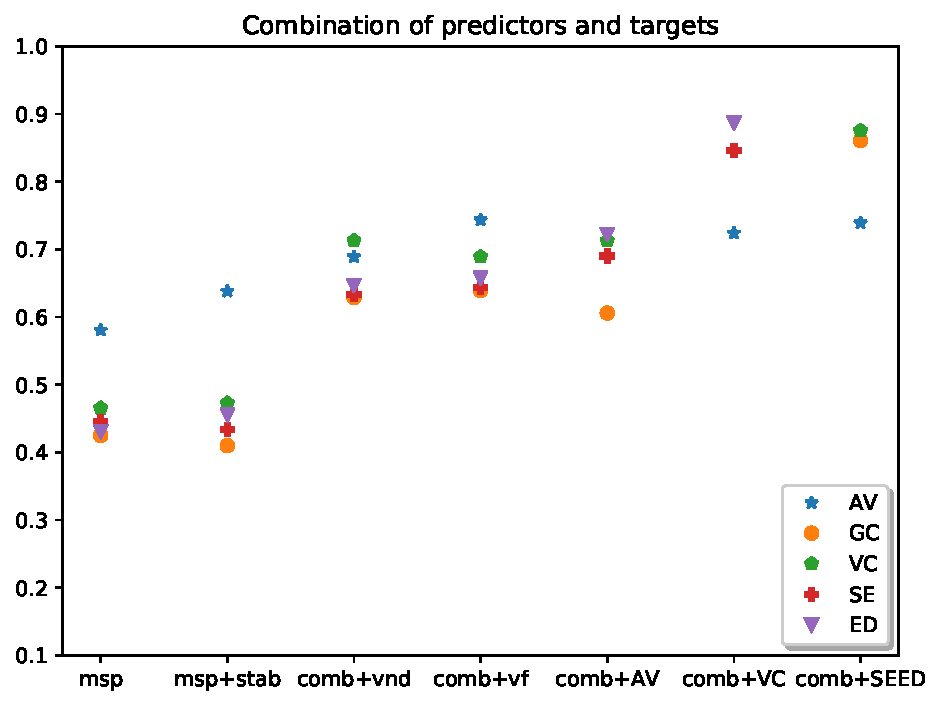
\includegraphics[width=\linewidth]{result/figures/comboofpred.pdf}
    \end{subfigure}%
        \caption{Li}
        \label{fig:predontarg_Li_last}
\end{figure}


For \textit{average voltage} ur best accuracy is around $73\%$ \ref{tab:Li-vnd-msp-vf-stability}, with an high accuracy, WAPE $= 4.2\%$. Which is not adequate for our ML model to be reliable on prediction of AV. The paper by Joshi \textit{et al.} \cite{joshi2019machine} made predictions on the same db, where they applied the features: the concentration of the active metal ion, crystal lattice types and space group numbers. They also adopted features from the work by Ward \textit{et al.} \cite{ward2016general}, where the elemental properties where added to the feature vector. 




\begin{comment}
\begin{figure}[h]
    \centering
    \begin{subfigure}{0.3\textwidth}
        \centering
        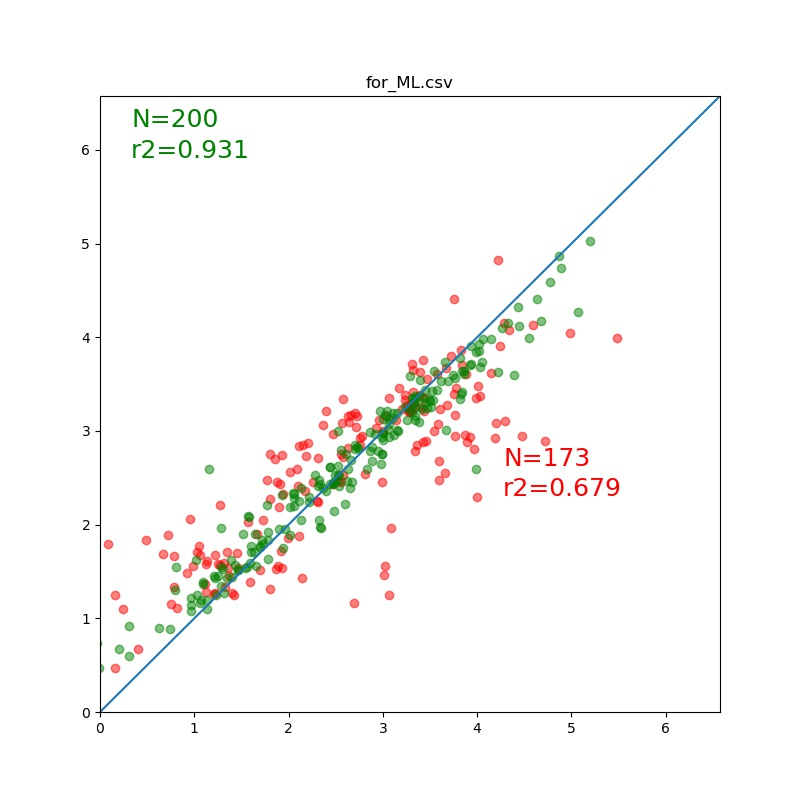
\includegraphics[width=\linewidth]{Results/2019-04-11/target=Average_Voltage.jpg}
        \caption{}
    \end{subfigure}
   % ~ 
    \begin{subfigure}{0.3\textwidth}
        \centering
        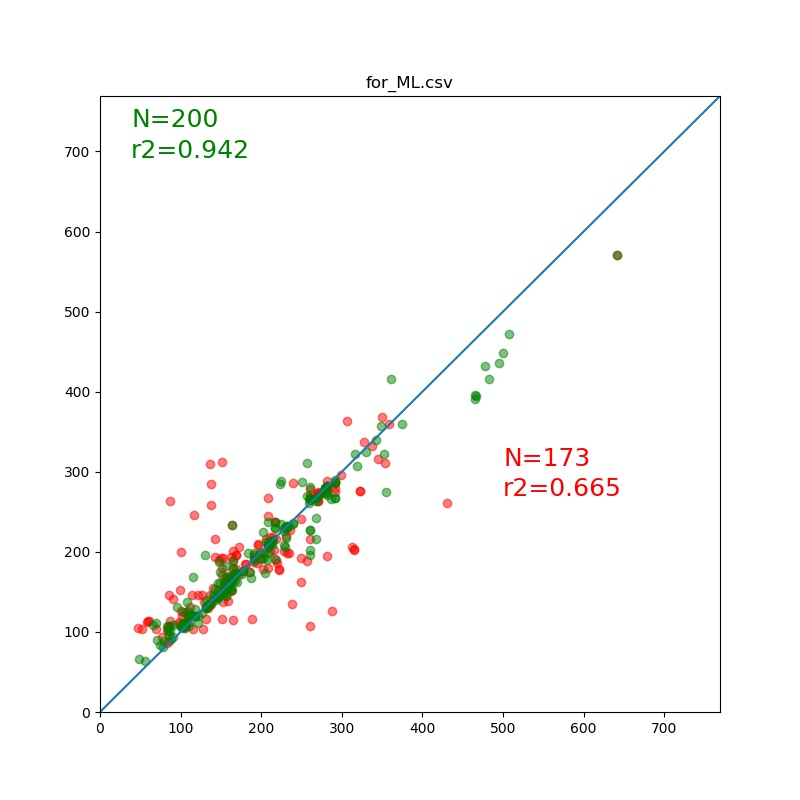
\includegraphics[width=\linewidth]{Results/2019-04-11/target=Capacity_Grav.jpg}
        \caption{}
    \end{subfigure}
       % ~ 
    \begin{subfigure}{0.3\textwidth}
        \centering
        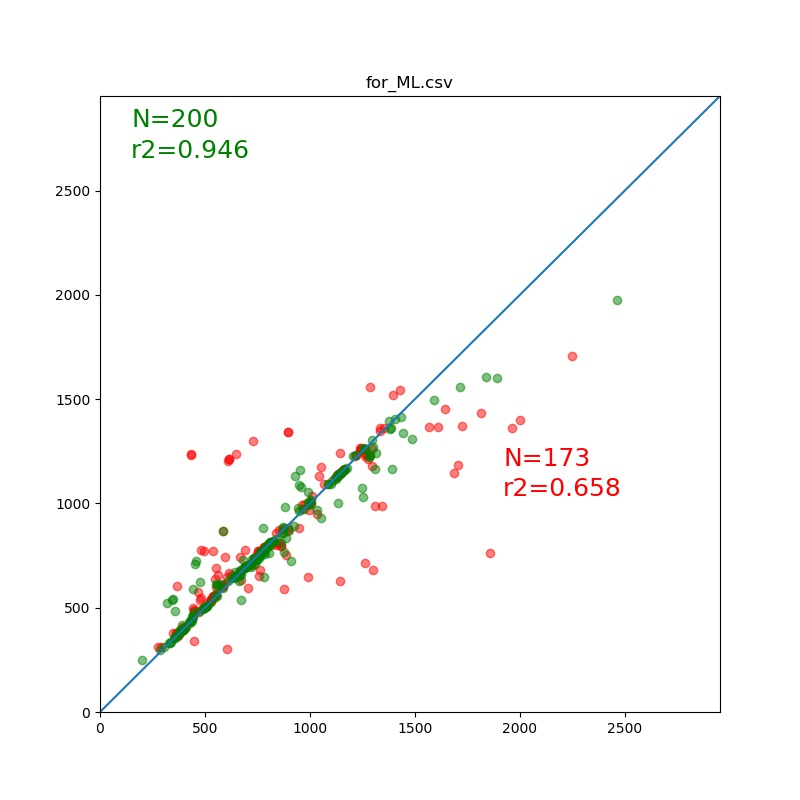
\includegraphics[width=\linewidth]{Results/2019-04-11/target=Capacity_Vol.jpg}
        \caption{}
    \end{subfigure}
       % ~ 
    \begin{subfigure}{0.3\textwidth}
        \centering
        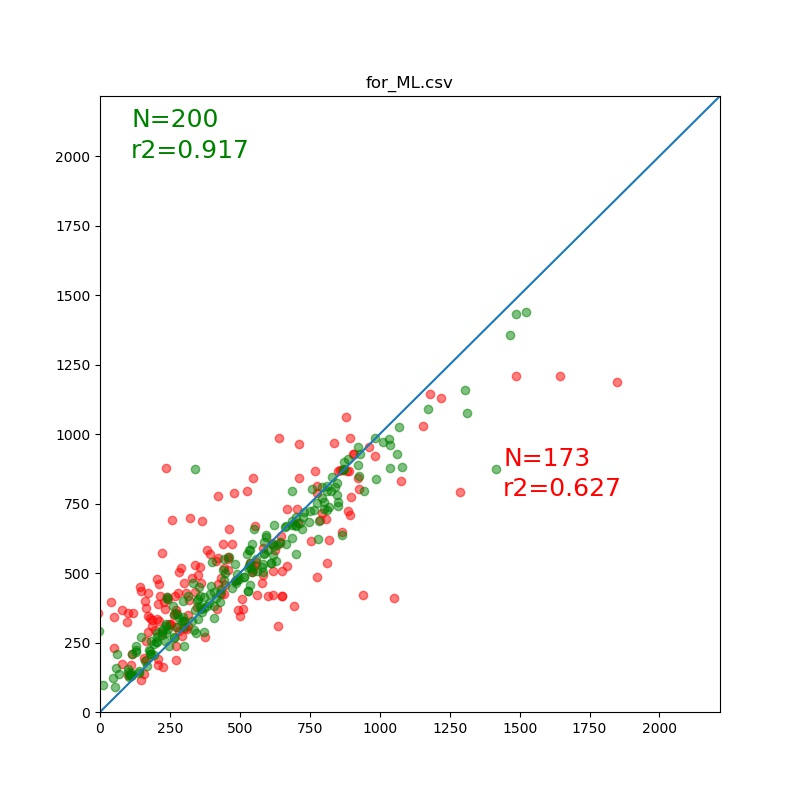
\includegraphics[width=\linewidth]{Results/2019-04-11/target=Specific_E_Wh_kg.jpg}
        \caption{}
    \end{subfigure}
       % ~ 
    \begin{subfigure}{0.3\textwidth}
        \centering
        \includegraphics[width=\linewidth]{Results/2019-04-11/target=E_Density_Wh_l.jpg}
            \caption{}
    \end{subfigure}
       % ~ 
    \begin{subfigure}{0.3\textwidth}
        \centering
        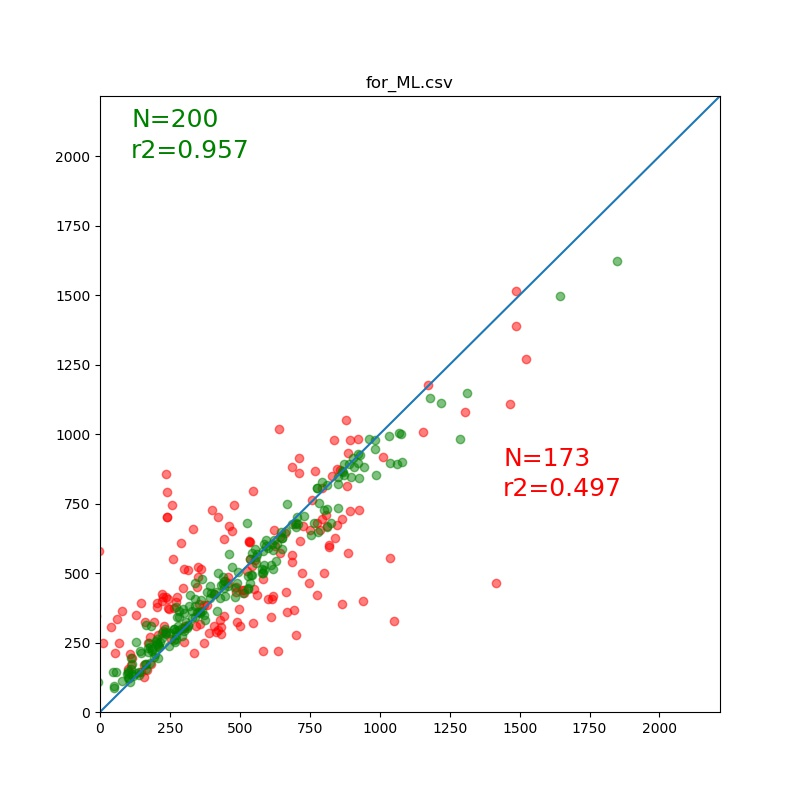
\includegraphics[width=\linewidth]{Results/2019-04-11/target=Stability_Discharge.jpg}
            \caption{}
    \end{subfigure}
\caption[R2 plot]{R2 plot for different runs}
    \label{fig:numberdensity_a-f}

\end{figure}

\subsection{Energy descriptions}

\begin{figure}
    \centering
    \includegraphics[width=\linewidth]{Results/plots/mean_crossvalidation_plot.png}
\caption[Cross validation and prediction uncertainty plot]{The Cross validation and the predictions uncertainty plottet for different runs with different predictors and the specific energy as the target for all runs. No removal of outliers have been implemented. l = number density, hgv = helvol, geomvol of void fraction, AV = average voltage, CGV = gravimetric and volumetric capacity, ED = energy density}
\label{fig:mean_cv}
\end{figure}
\myworries{}
\end{comment}


%Parameters.
%Volume number density
%Try to tell a STORY.


%Presentation between 30-45 minuttes. 

%Problem?
%method
%solution? 

% Test with density fraction:


% Test; weight of different parameters.















